\chapter{Results and discussion}\label{chap:Results&Disc}
In this chapter the results and methods from laboratory experiments are presented and discussed.

\section{PFCA sorption behavior}
\subsection{Biochar-water sorption isotherms}
In \cref{fig:sorption_isotherms}, the sorption isotherms are presented for PFPeA, PFHxA, PFHpA, PFOA, PFNA and PFDA to CWC, ULS and DSL. The points generated from the batch tests were fitted using the Freundlich model (\cref{eq:FreundlichLinear}). For all compounds, the sorption isotherm for ULS is visibly higher than DSL, followed by CWC. The Freundlich sorption coefficients ($log~K_F$), linearity coefficients ($n_F$) and correlation coefficients ($r^2$) are presented in \cref{tab:summary_stats_single}. Somewhat unexpectedly, sorption is strongest for the two sludge chars. Possible mechanisms for the strong sorption will be discussed in this section. 

Due to the pioneering research on sewage sludge biochars as sorbents for PFAS in this thesis, literature partitioning coefficients for PFCAs of other sewage sludge biochars are non-existent (is that correct?). However, a comparison can be made between the $log~K_F$s found in this thesis and for commercially-produced activated carbons (AC) reported in other studies. The sorption coefficients are equivalent or higher compared to literature values for $log~K_F$ of PFOA to AC: 5.60 \citep{Kupryianchyk2016a}, 4.45 \citep{hansen2010sorption}, and 4.74-5.42 \citep{silvani2019can}. This is promising for the potential to replace non-renewable AC with waste based biochars for environmental remediation in the field and wastewater treatment. 

\begin{figure}[tb]
    \centering
    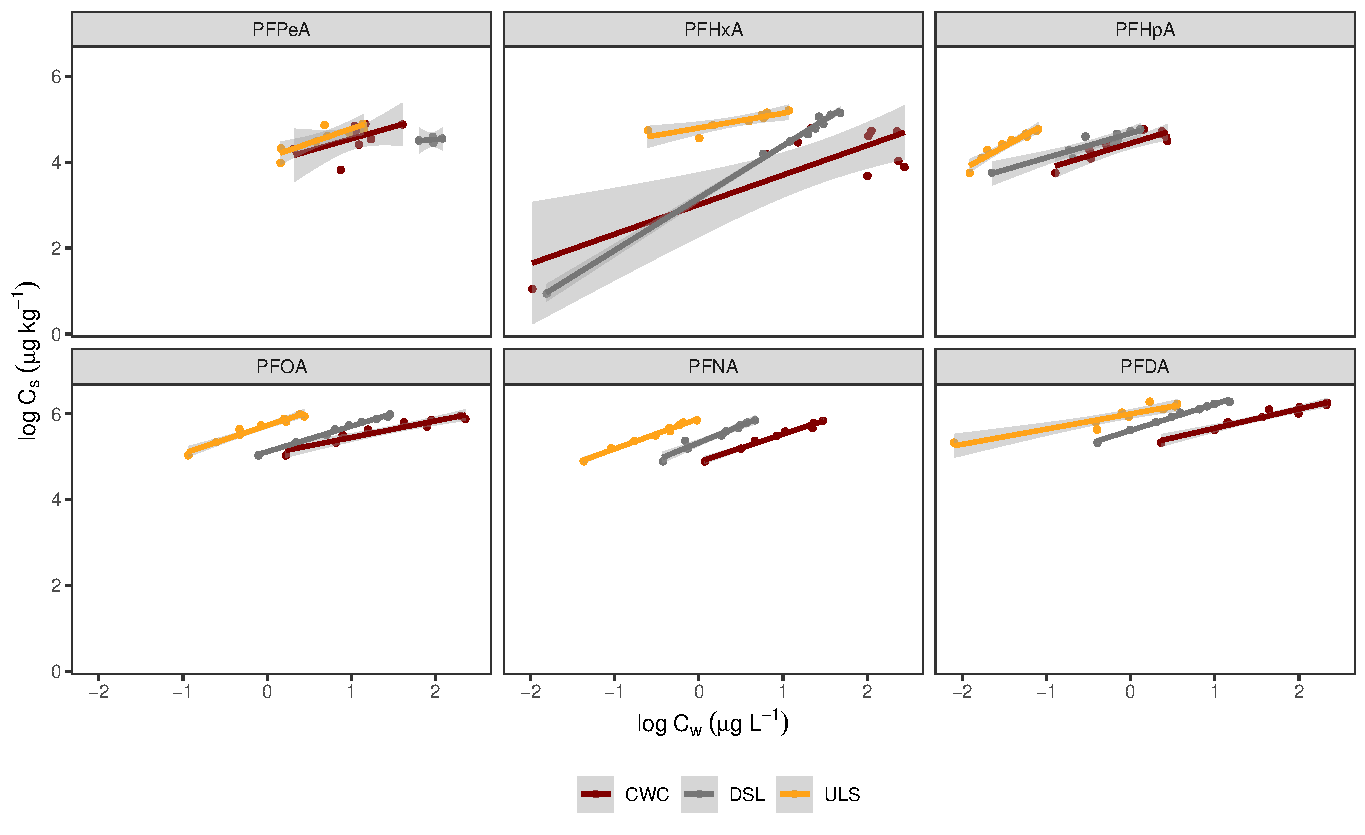
\includegraphics[width=\textwidth]{R/figs/Sorption_isotherms_single_BC.pdf}
    \caption{Freundlich sorption isotherms of TCs in batch tests with three different biochars. Lines are obtained by linear regression.}
    \label{fig:sorption_isotherms}
\end{figure}

\begin{table}
\caption{Freundlich sorption parameters of single TC isotherms in CWC, ULS and DSL (n=9). The error is presented as standard error. All $K_F$ data are in units of $\mathrm{(\mu g/kg)/(\mu g/L)^{n_F}}$.}
\centering
\adjustbox{max width=\textwidth}{%
\begin{threeparttable}
\label{tab:summary_stats_single}
\begin{tabular}{lllllllllllll} \toprule
PFCA & \multicolumn{4}{c}{ULS} & \multicolumn{4}{c}{DSL} & \multicolumn{4}{c}{CWC} \\ \cmidrule(l){2-5} \cmidrule(l){6-9} \cmidrule(l){10-13}
 & $log~K_{F,BC}$ & $n_{F,BC}$ & $r^2$ & $p$ & $log~K_{F,BC}$ & $n_{F,BC}$ & $r^2$ & $p$ & $log~K_{F,BC}$ & $n_{F,BC}$ & $r^2$ & $p$ \\ \midrule
PFPeA & 4.10 ± 0.13 & 0.67 ± 0.16 & 0.74 & ** & 4.25 ± 0.74 & 0.14 ± 0.38 & 0.06 & $>$0.05 & 3.98 ± 0.36 & 0.56 ± 0.33 & 0.30 & $>$0.05 \\
PFHxA & 4.80 ± 0.06 & 0.34 ± 0.09 & 0.72 & ** & 3.30 ± 0.15 & 1.11 ± 0.11 & 0.93 & *** & 4.59 ± 0.50 & -0.14 ± 0.26 & 0.04 & $>$0.05 \\
PFHpA & 5.98 ± 0.17 & 1.08 ± 0.11 & 0.93 & *** & 4.67 ± 0.06 & 0.57 ± 0.09 & 0.86 & *** & 4.44 ± 0.05 & 0.59 ± 0.11 & 0.80 & ** \\
PFOA & 5.73 ± 0.02 & 0.65 ± 0.05 & 0.95 & *** & 5.12 ± 0.02 & 0.60 ± 0.02 & 0.99 & *** & 5.06 ± 0.08 & 0.39 ± 0.05 & 0.90 & *** \\
PFNA & 5.89 ± 0.02 & 0.71 ± 0.03 & 0.99 & *** & 5.33 ± 0.03 & 0.80 ± 0.07 & 0.94 & *** & 4.88 ± 0.04 & 0.65 ± 0.04 & 0.98 & *** \\
PFDA & 6.00 ± 0.04 & 0.35 ± 0.05 & 0.86 & *** & 5.61 ± 0.02 & 0.61 ± 0.02 & 0.99 & *** & 5.22 ± 0.07 & 0.45 ± 0.04 & 0.94 & *** \\ \bottomrule
\end{tabular}
\begin{tablenotes}
\item Significant codes: *** $\sim$ 0.001, ** $\sim$ 0.01  
\end{tablenotes}
\end{threeparttable}}
\end{table}

\subsection{Effect of PFCA properties}
\subsubsection{PFCA chain length}
\cref{fig:sorption_isotherms_all} shows sorption isotherms for the single-compound batch tests for CWC, ULS and DSL. The Freundlich coefficients for ULS increased in the order, PFPeA $<$ PFHxA $<$ PFOA $<$ PFHpA $<$ PFNA $<$ PFDA, ranging from $log~K_F$ = 4.10-6.00 (\cref{tab:summary_stats_single}). All regressions were significant (p$<$0.01). The Freundlich coefficients for DSL increased in the order, PFHxA $<$ PFPeA $<$ PFHpA $<$ PFOA $<$ PFNA $<$ PFDA, ranging from $log~K_F$ = 3.16-5.61. All regressions were significant (p$<$0.001) except for the PFPeA isotherm which only consisted of four points (SP7-10) due to higher analyzed filtrate concentrations than what was spiked for SP1-6 (attributed to analytical uncertainty or imprecision/contamination during laboratory work) (\cref{fig:DSL_isotherm}). The Freundlich coefficients for CWC increased in the order, PFPeA $<$ PFHpA $<$ PFHxA $<$ PFNA $<$ PFOA $<$ PFDA, ranging from $log~K_F$ = 3.01-5.22. All regressions were significant (p$<$0.01) except for PFPeA and PFHxA despite nine points used in the regressions. Changes in $log~K_F$ with chain length can be visualized in \cref{subfig:chainlength}. 

A statistically significant relationship between $log~K_F$ and CF\textsubscript{2} chain length was found for all three biochars (p$<$0.05, \cref{fig:chain_length_n}), which is in accordance with previous studies \citep{Sorengard2019,higgins2006sorption,ahmed2020per}. There was a difference of 1.2-1.9 $log~K_F$ units between the longest and the shortest PFCA chain (PFDA and PFPeA). For every CF\textsubscript{2} moiety, hydrophobic interactions between condensed aromatic structures in the biochar matrix increases, contributing to stronger sorption. Several mechanisms can be used to explain why perfluorinated carboxylic acids increase in hydrophobicity with increasing chain length. 1) Due to high molecular surface of the perfluorinated tail, a high cavity formation energy is needed to dissolve the compounds in water, and therefore they tend to be pushed towards water extremities, such as a biochar surface. Therefore, dissolution becomes increasingly energetically demanding with increasing chain length \citep{sigmund2022sorption}. 2) the perfluorinated chain with CF\textsubscript{2} moieties is capable of the least van der Waals interactions per molecular surface area compared to CH\textsubscript{2} which results in the least interactions between water molecules when in the water cavity. This is why PFASs are both oil- and water repellent. 

\begin{figure*}[htb]
    \centering
    \begin{subfigure}[t]{0.45\textwidth}
        \centering
        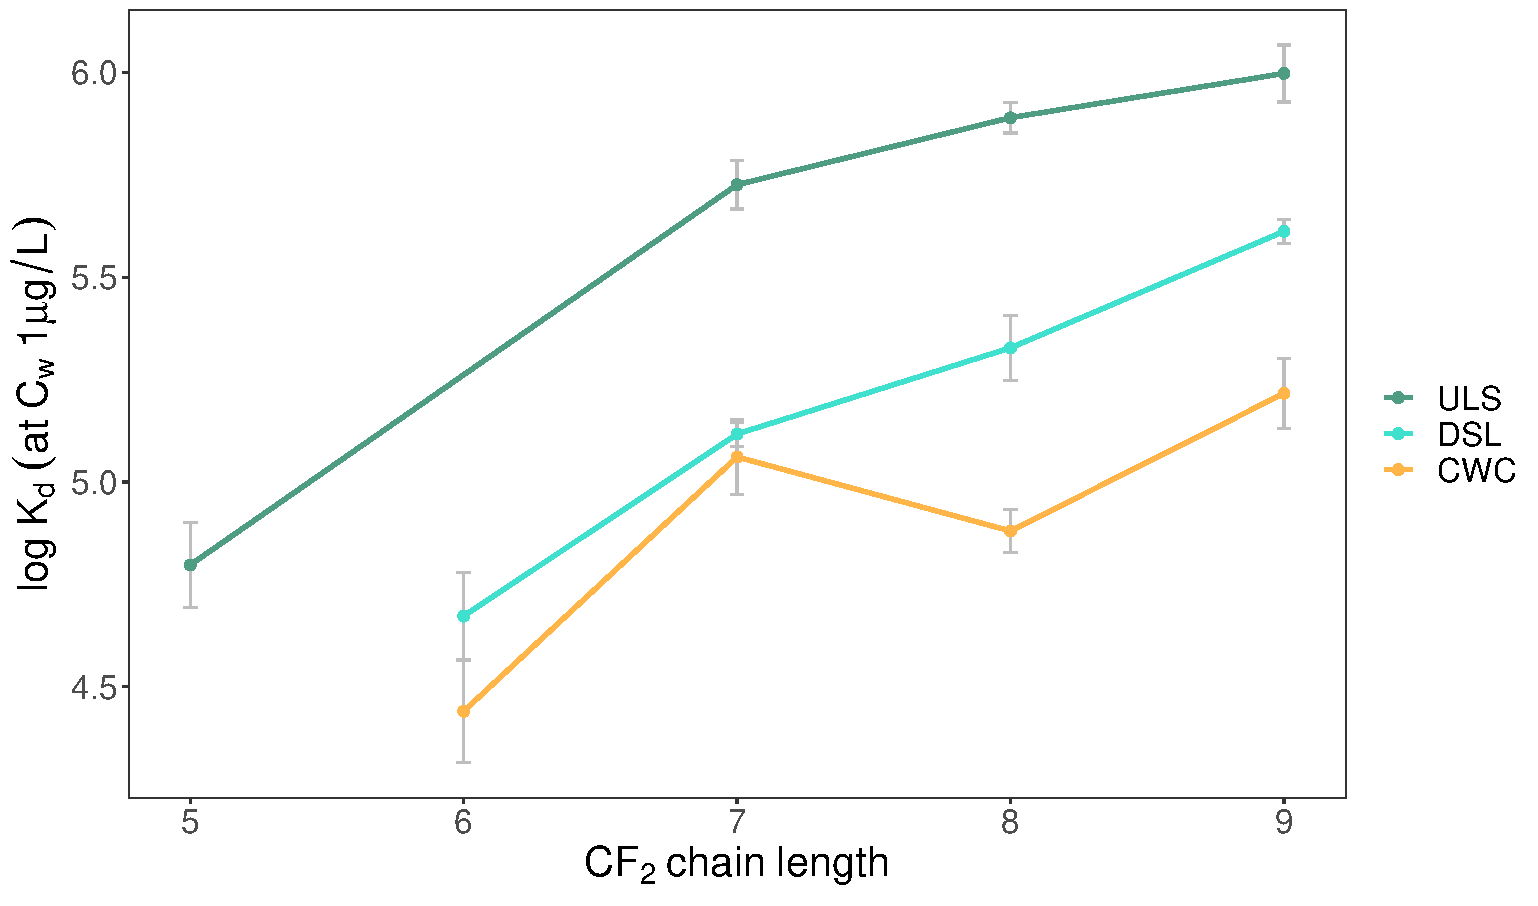
\includegraphics[width=\textwidth]{R/figs/chain_length_Kd1ugL_plot.pdf}
        \caption{}
        \label{subfig:chainlength}
    \end{subfigure}%
    ~ 
    \begin{subfigure}[t]{0.45\textwidth}
        \centering
        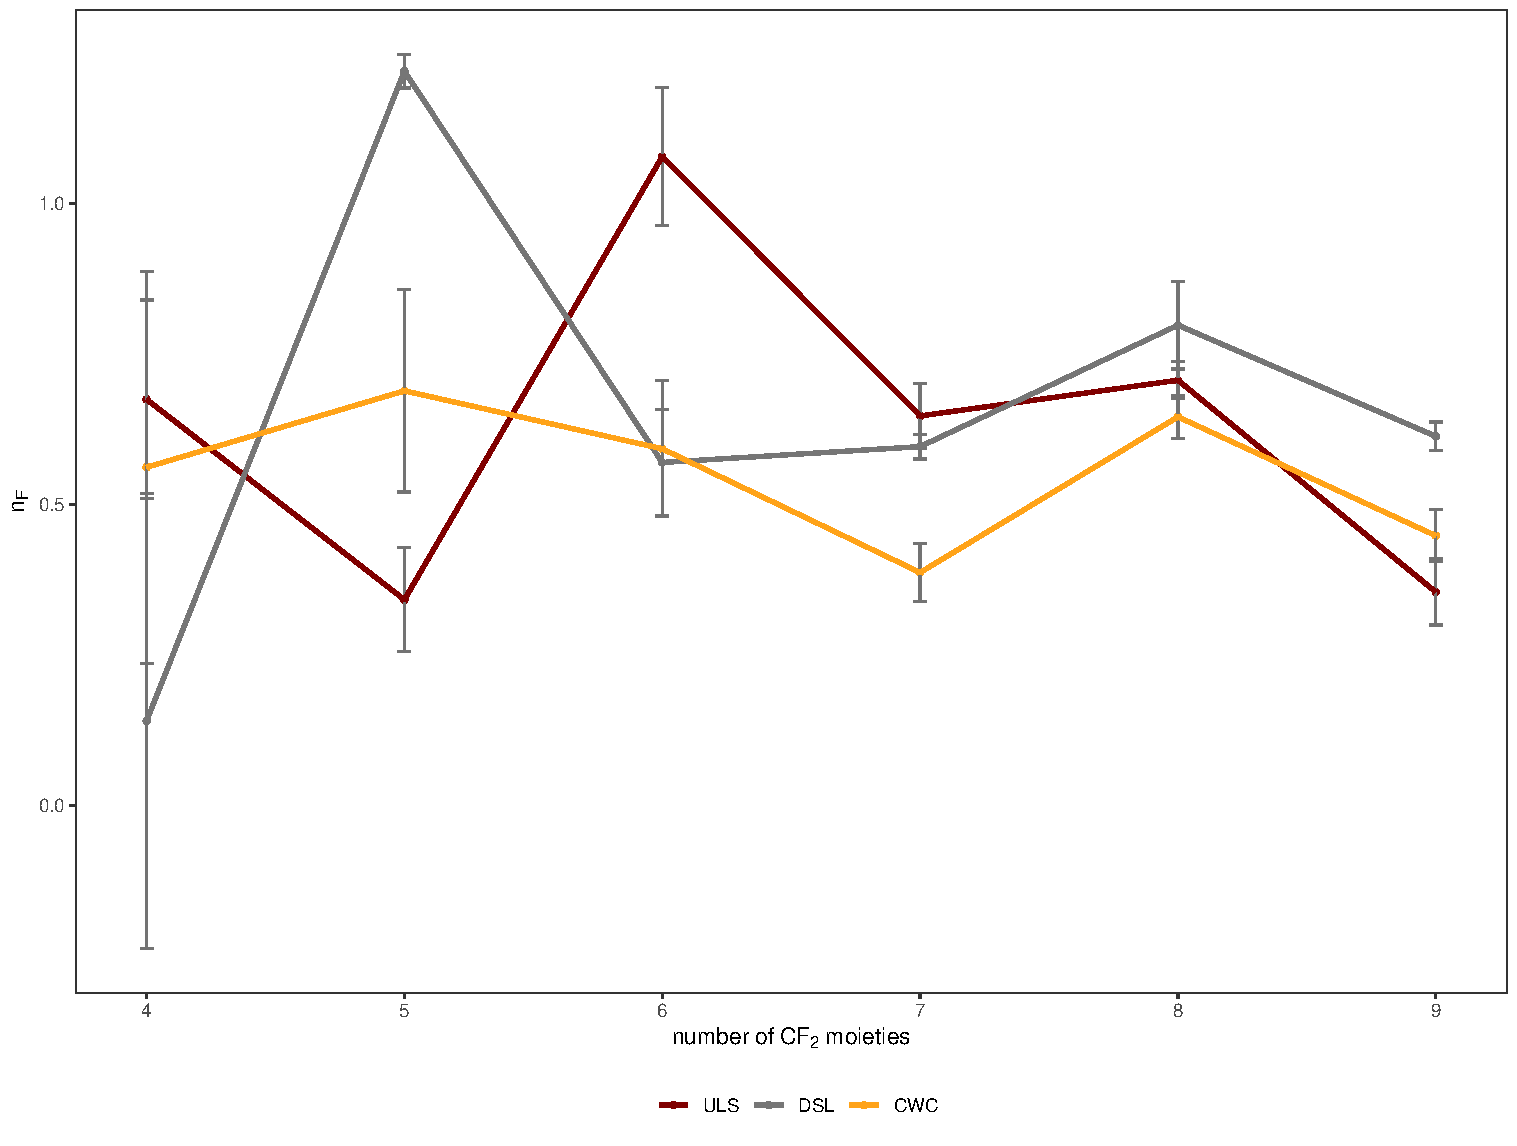
\includegraphics[width=\textwidth]{R/figs/n_KF.pdf}
        \caption{}
        \label{subfig:n}
    \end{subfigure}
    \label{fig:chain_length_n}
    \caption{Relationship between \textbf{(a)} Correlation between $log~K_F$ and chain length. Linear regression coefficients for ULS: $r^2$ = 0.68, $p$ = 0.52, DSL: $r^2$ = 0.98, $p$ = 0.012, CWC: $r^2$ = 0.93, $p$ = 0.007. Error bars are the propagated error of $log~K_F$ and $n_F$. \textbf{(b)} $n_F$ and $CF_2$ chain length. Error bars are the standard error of $log~K_F$ for each chain length and biochar isotherm.}
\end{figure*}

\begin{figure}
    \centering
        \begin{subfigure}[]{\linewidth}
            \centering
            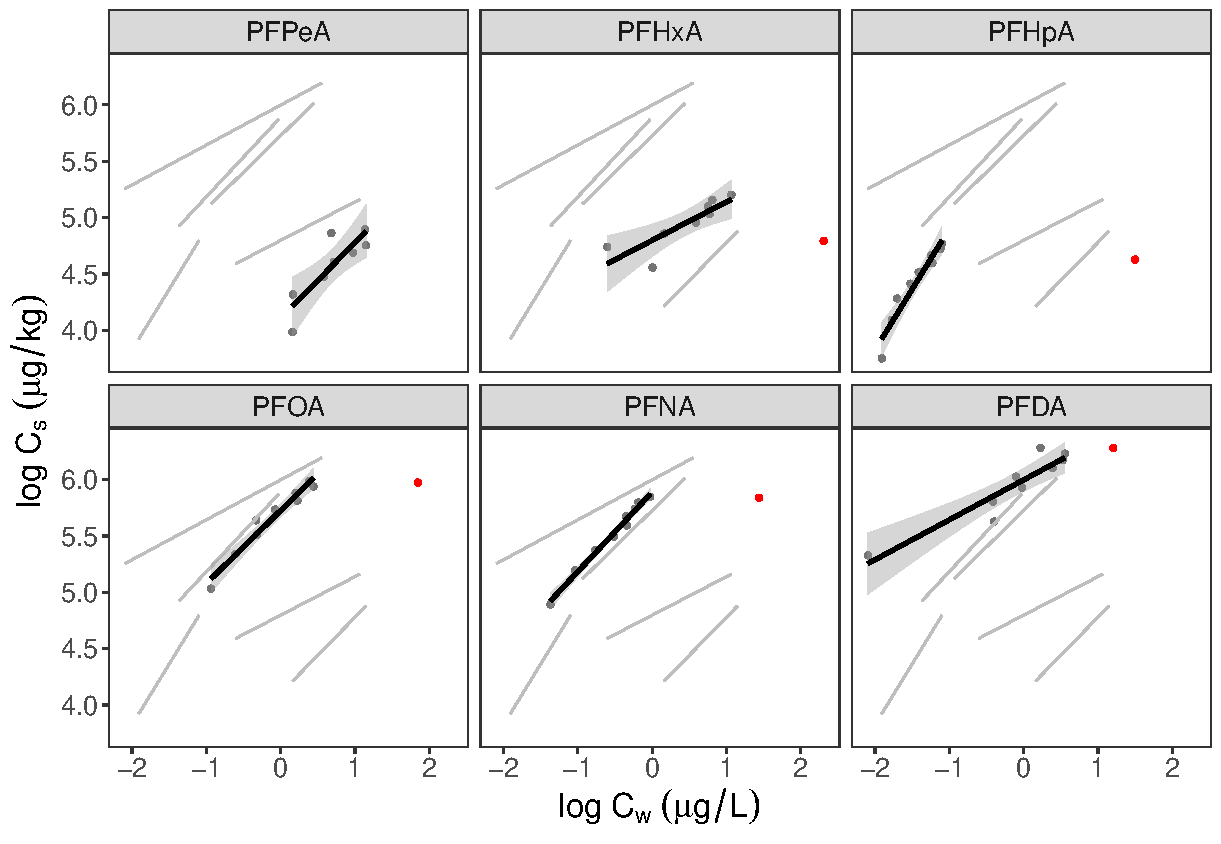
\includegraphics[width=0.6\textwidth]{R/figs/ULS_facet_isotherm.pdf}
            \subcaption{ULS isotherms}
            \label{fig:ULS_isotherm}
        \end{subfigure}
        \begin{subfigure}[]{\linewidth}
            \centering
            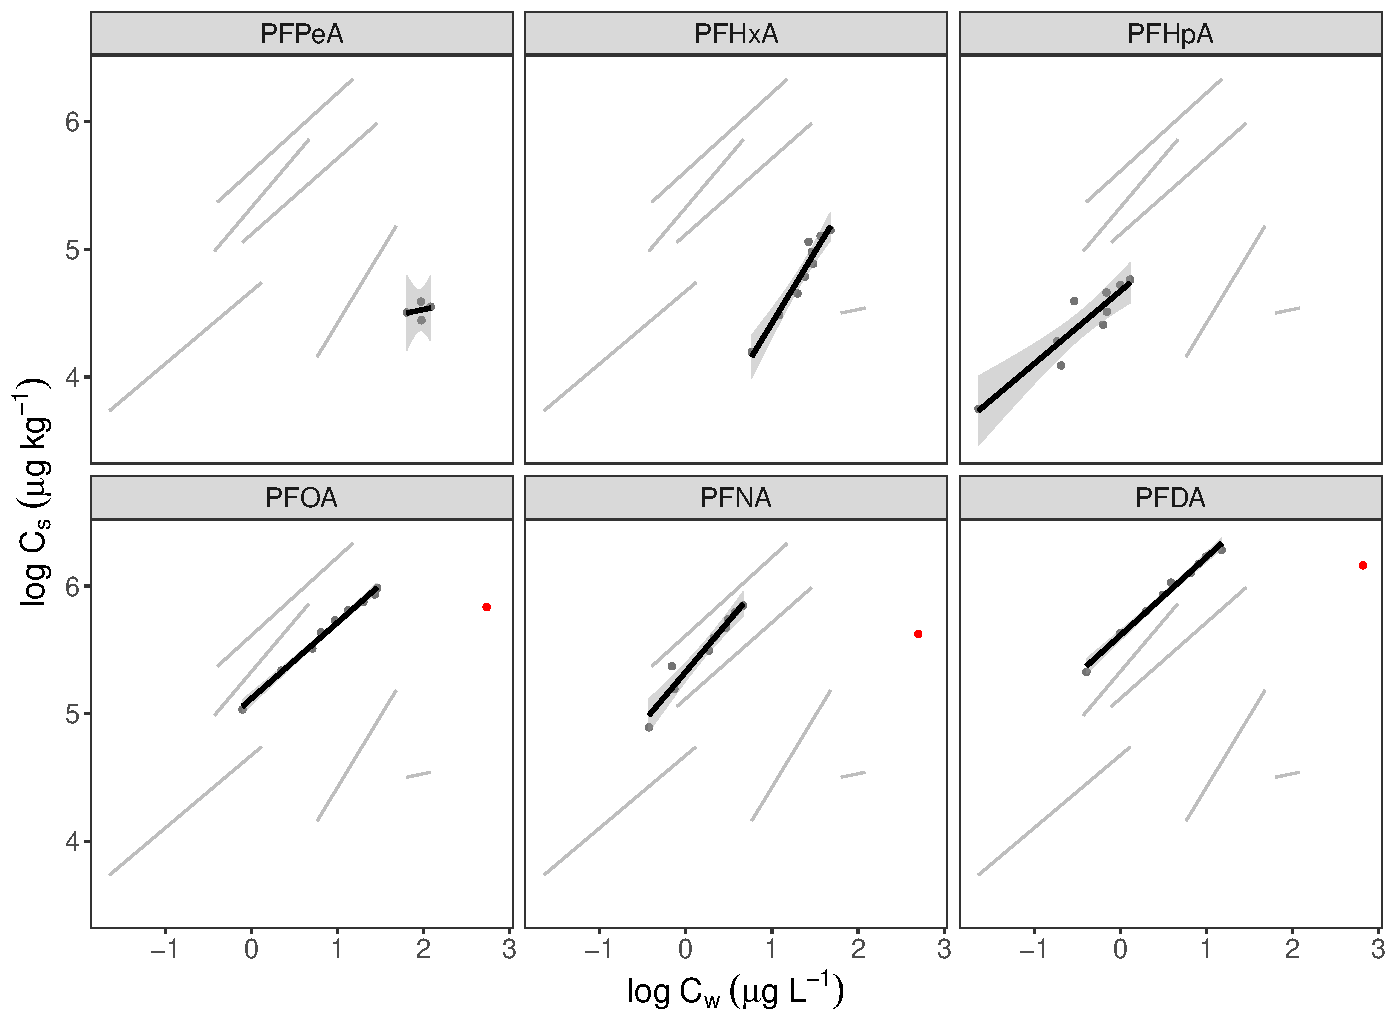
\includegraphics[width=0.6\textwidth]{R/figs/DSL_facet_isotherm.pdf}
            \subcaption{DSL isotherms}
            \label{fig:DSL_isotherm}
        \end{subfigure}   
\end{figure}
\begin{figure}[t]\ContinuedFloat
        \begin{subfigure}[]{\linewidth}
            \centering
            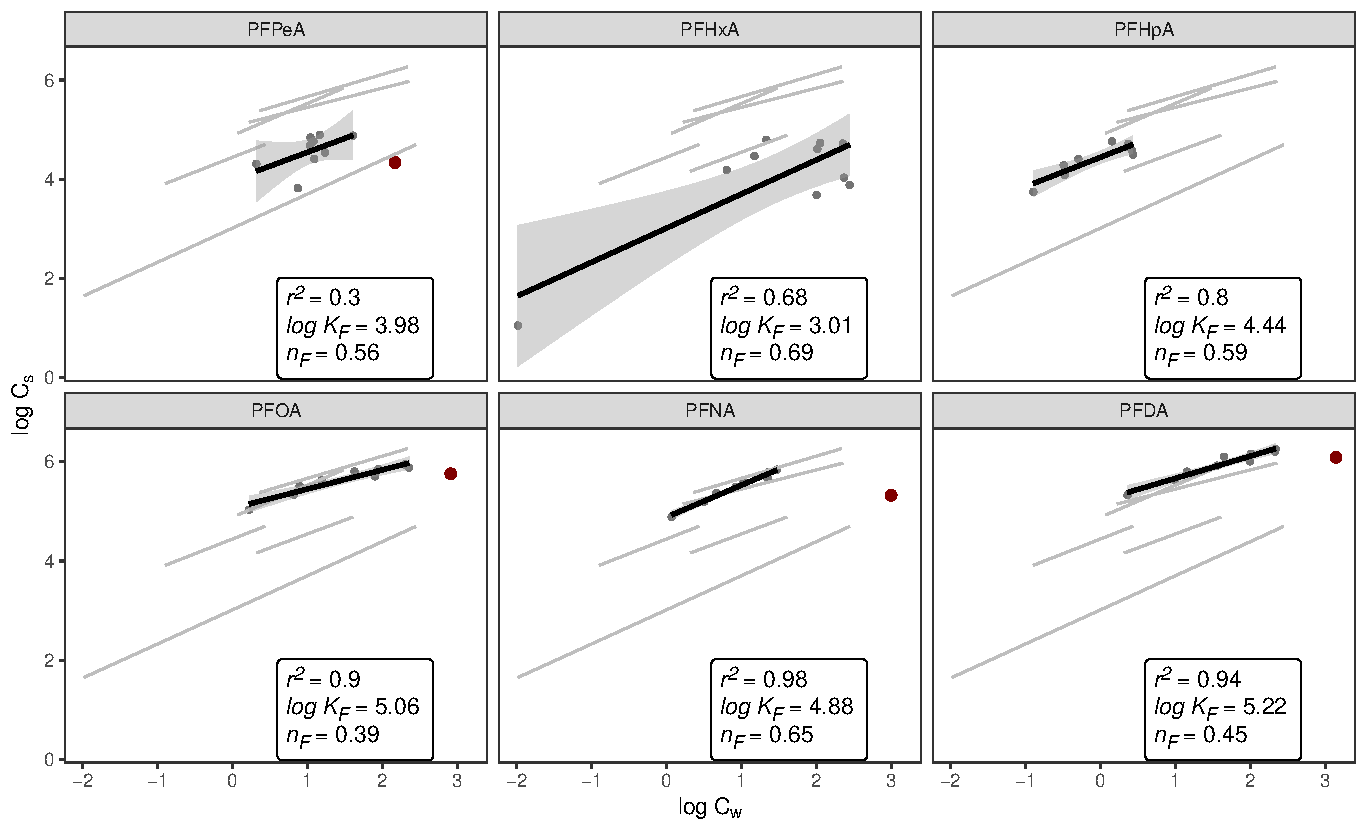
\includegraphics[width=0.6\textwidth]{R/figs/CWC_facet_isotherm.pdf}
            \subcaption{CWC isotherms}
            \label{fig:CWC_isotherm}
        \end{subfigure}
        \caption{Single-compound Freundlich sorption isotherms of PFPeA, PFHxA, PFHpA, PFOA, PFNA and PFDA. Lines are obtained by linear regression.}
        \label{fig:sorption_isotherms_all}
\end{figure}

\subsubsection{PFAS functional group} 
The charged and polar head of PFCAs give these compound classes unique sorptive properties because the polar head can engage simultaneously in electrostatic bonding with surface functional groups or bridging cations within the biochar matrix (ash rich in cations) \citep{zhang2013sorption,sigmund2022sorption}. In this study, the highest sorption were seen for ULS and DSL with the lowest \% C (\cref{tab:SAPV}), which is in contrast with previous literature. However, previous PFAS sorption studies have been conducted on biochar from cleaner, wood-based feedstock \citep{Sormo2021}, activated carbon \citep{zhang2021sorption,Kupryianchyk2016b}, soils and sediments \citep{higgins2006sorption}, and raw sewage sludges \citep{zhang2013sorption}. These studies conclude that the importance of electrostatic interaction to sorption comes secondary to the hydrophobic effect. The main reason for this is that the biochar surface is net negatively charged with a high cation exchange capacity (CEC) \citep{Ahmad2014} and may experience electrostatic repulsion of the negatively charged functional group on the PFAS (Include PZC when available). PFCAs have low $pK_a$s (-1, \citep{goss2008pKa}) due to having strong electron withdrawing fluorine atoms and hence become strong acids. The PFCAs investigated in this study will be negatively charged given the filtrate pH of 7.1-7.4 (\cref{tab:pHcond}). Thus, all TCs experience electrostatic repulsion from the biochar surface which result in the lowest $K_F$-values for the shorter-chain PFCAs (\cref{tab:summary_stats_single}). Electrostatic repulsion is reduced in acid soils where the CEC is reduced and the biochar surfaces become protonated and more neutral. This allows for anion- \textpi bond interaction with biochar \citep{sigmund2022sorption}. 

\cite{zhang2021sorption} found that sorption increased in the order PFBA $<$ PFBS $<$ PFOA $<$ PFOS for granular activated carbon and softwood-derived biochar. The difference between the PFSA and PFCA groups is that PFSAs have one more perfluorinated carbon than PFCAs, which has its terminal carbon bonded as a carboxylate (COO\textsuperscript{-}). If one compares PFHpS with PFOA, which have the same number of $\mathrm{CF_2}$ moieties, the perfluorinated sulfonic acid still sorbs better. Researchers attribute this to 1) difference in molecular size, where the sulfonate moiety is slightly larger than the carboxylate moiety, which results in greater cavity formation energy of PFSAs, and hence in water saturated conditions, the functional group is pushed towards water extremities \citep{yin2022insights,sigmund2022sorption}. In batch shaking experiments this would be the biochar surfaces or tube walls; 2) Because sulfonic acid is a stronger acid than carboxylic acid which results in stronger ionic interaction to positive charges of mineral phases \citep{arvaniti2015review}. \cite{du2014adsorption}: electr and hydry balance Since sorption increased with chain length onto all three biochars in this study, this suggests that hydrophobic interactions is the dominant sorption mechanism over electrostatic interactions. Therefore, further investigation to explain why the sludge biochars sorb better than CWC will follow. 

%%%%%%%%%%%%%%%%%%%%%%%%%%%%%%%%%%%%%%%%%%%%%%%%%%%%%%%%%%%%%%%%%%%%%%%%%%%%%%%%%%%%%%%%%%%%%%%%%%%%%%%%%%%%%%%%%%%%%%%%%%%%%%%%%%%%%%%%%%%%%%%%%%%%%%%%%%%%%%%%%%%%%%%%%%%%%%%%%%%%%%%%%%%%%%%%%%%%%%%%%%%%%%%%%%%%%%%%%%%%%%%%%%%%%%%%%%%%%%%%%%%%%%%%%%%%%%%%%%%%%%%%%%%%%%%%%%%%%%%%%%%%%%%%%%%%%%%%%%%%%%%%%%%%%%%%%%%%%%%%%%%%%%%%%%%%%%%%%%%%%%%%%%%%%%%%%%%%%%%%%%%%%%%%%%%%%%%%%%%%%%%%%%%%%%%%%%%%%%%%%%%%%%%%%%%%%%%%%%%%%%%%%%%%%%%%%%%%%%%%%%%%%%%%%%%%%%%%%%%%%%%%%%%%%%%%%%%%%%%%%%%%%%%%%%%%%%%%%%%%%%%%%%%%%%%%%%%%%%%%%%%%%%%%%%%%%%%%%%%%%%%%

\section{Sorption attenuation by soil and competing congeners}
Table with partitioning coefficients for the biochar sorbents with and without the presence of soil, plus/minus standard error
Kd at C10 for soil alone
How to account for Kd of soil when calculating KF 
    Show how to derive Freundlich equation with respect to soil Kd from original Freundlich equation

\cref{fig:C10} shows the $K_d$ values for the different batch test categories spiked at SC10 for each compound (\cref{tab:spikeConcentrations}, note: $K_d$-values cannot be compared between compounds as different spike concentrations were used). The figure shows that sorption is clearly attenuated by soil and competing congeners as the BC single points are highest for all compounds. 

A table of attenuation factors for each batch test category is provided in \cref{apptab:attenuation}.

\subsection{Attenuation by competing congeners}

\subsection{Attenuation by soil}
The soil used in the batch tests was characterized as a fine sand (0.1 to 0.3 mm) with 1.3 \% TOC (pH 5.38 \textpm 0.02, CEC 2.63 \textpm 0.06 meqv 100 g\textsuperscript{-1}). Total element concentrations and exchangeable ion concentrations are in \cref{appSec:elements}, \cref{apptab:soil}. 

Soil extraction showed no native target analytes present. Upon filtration, each batch test category was different in its ease of filtration due to various degree of suspended particles and had different color filtrate, as seen in \cref{subfig:filtrate}. Filter clogging and reduction in filter pore size, had to exchange filters during filtration, which is a potential source of error. 

Aggregation of humic substances upon addition of acetic acid pre-SPE, how this may impact results. 

Precipitation of a brown fluff was observed when filtered batch tests containing soil was adjusted to pH 3 with 1 M acetic acid

Sorptive attenuation of a spiked cocktail of the six TCs were tested for each biochar is shown by the red point in \cref{fig:sorption_isotherms_all}. Due to different spike concentration used for each compound in the cocktail, establishing quantitative trends for how chain length influences competition for sorption size is difficult. However, some conclusions can be drawn by looking at the overall trends. \cref{tab:competition} shows that $log~K_d$ decreases for all compounds in the presence of a mixture. $K_d$ changes the least for PFHxA and PFHpA (2.3 and 0.2 \% respectively) and may be attributed to lower spiked concentrations (330 and 117 \textmu g L\textsuperscript{-1}) for these compounds compared to the rest in \cref{tab:competition}. Competition is most profound for PFOA to CWC followed by PFDA for ULS and CWC (15.8, 10.0 and 10.6 \% respectively), which can be explained by the highest concentrations spiked for these compounds (1 953 and 3 830 \textmu g L\textsuperscript{-1}). It appears that sorption of PFNA is minimally influenced by competition between other compounds despite SC being in the higher range (1 409 \textmu g L\textsuperscript{-1}). $K_d$ for PFPeA is reduced by 8.2\% and is expected based on weaker sorption of short-chain compounds.

Expected: Attenuation factors larger for short-chain than long chains which have greater sorption affinity.

Most previous studies have reported a linear increasing trend between log Kd and chain length. However not for PFPeA, \citep{zhang2013sorption}, found in \citep{Sorengard2019}. and \citep{guelfo2013}  these studies are for sorption to organic matter.  Steric hindrance. Competing sorption to humic matter
fouling/pre-loading by NOM
Pore blocking

\begin{figure}[htb]
\subfloat[\label{subfig:filtrate}]{%
  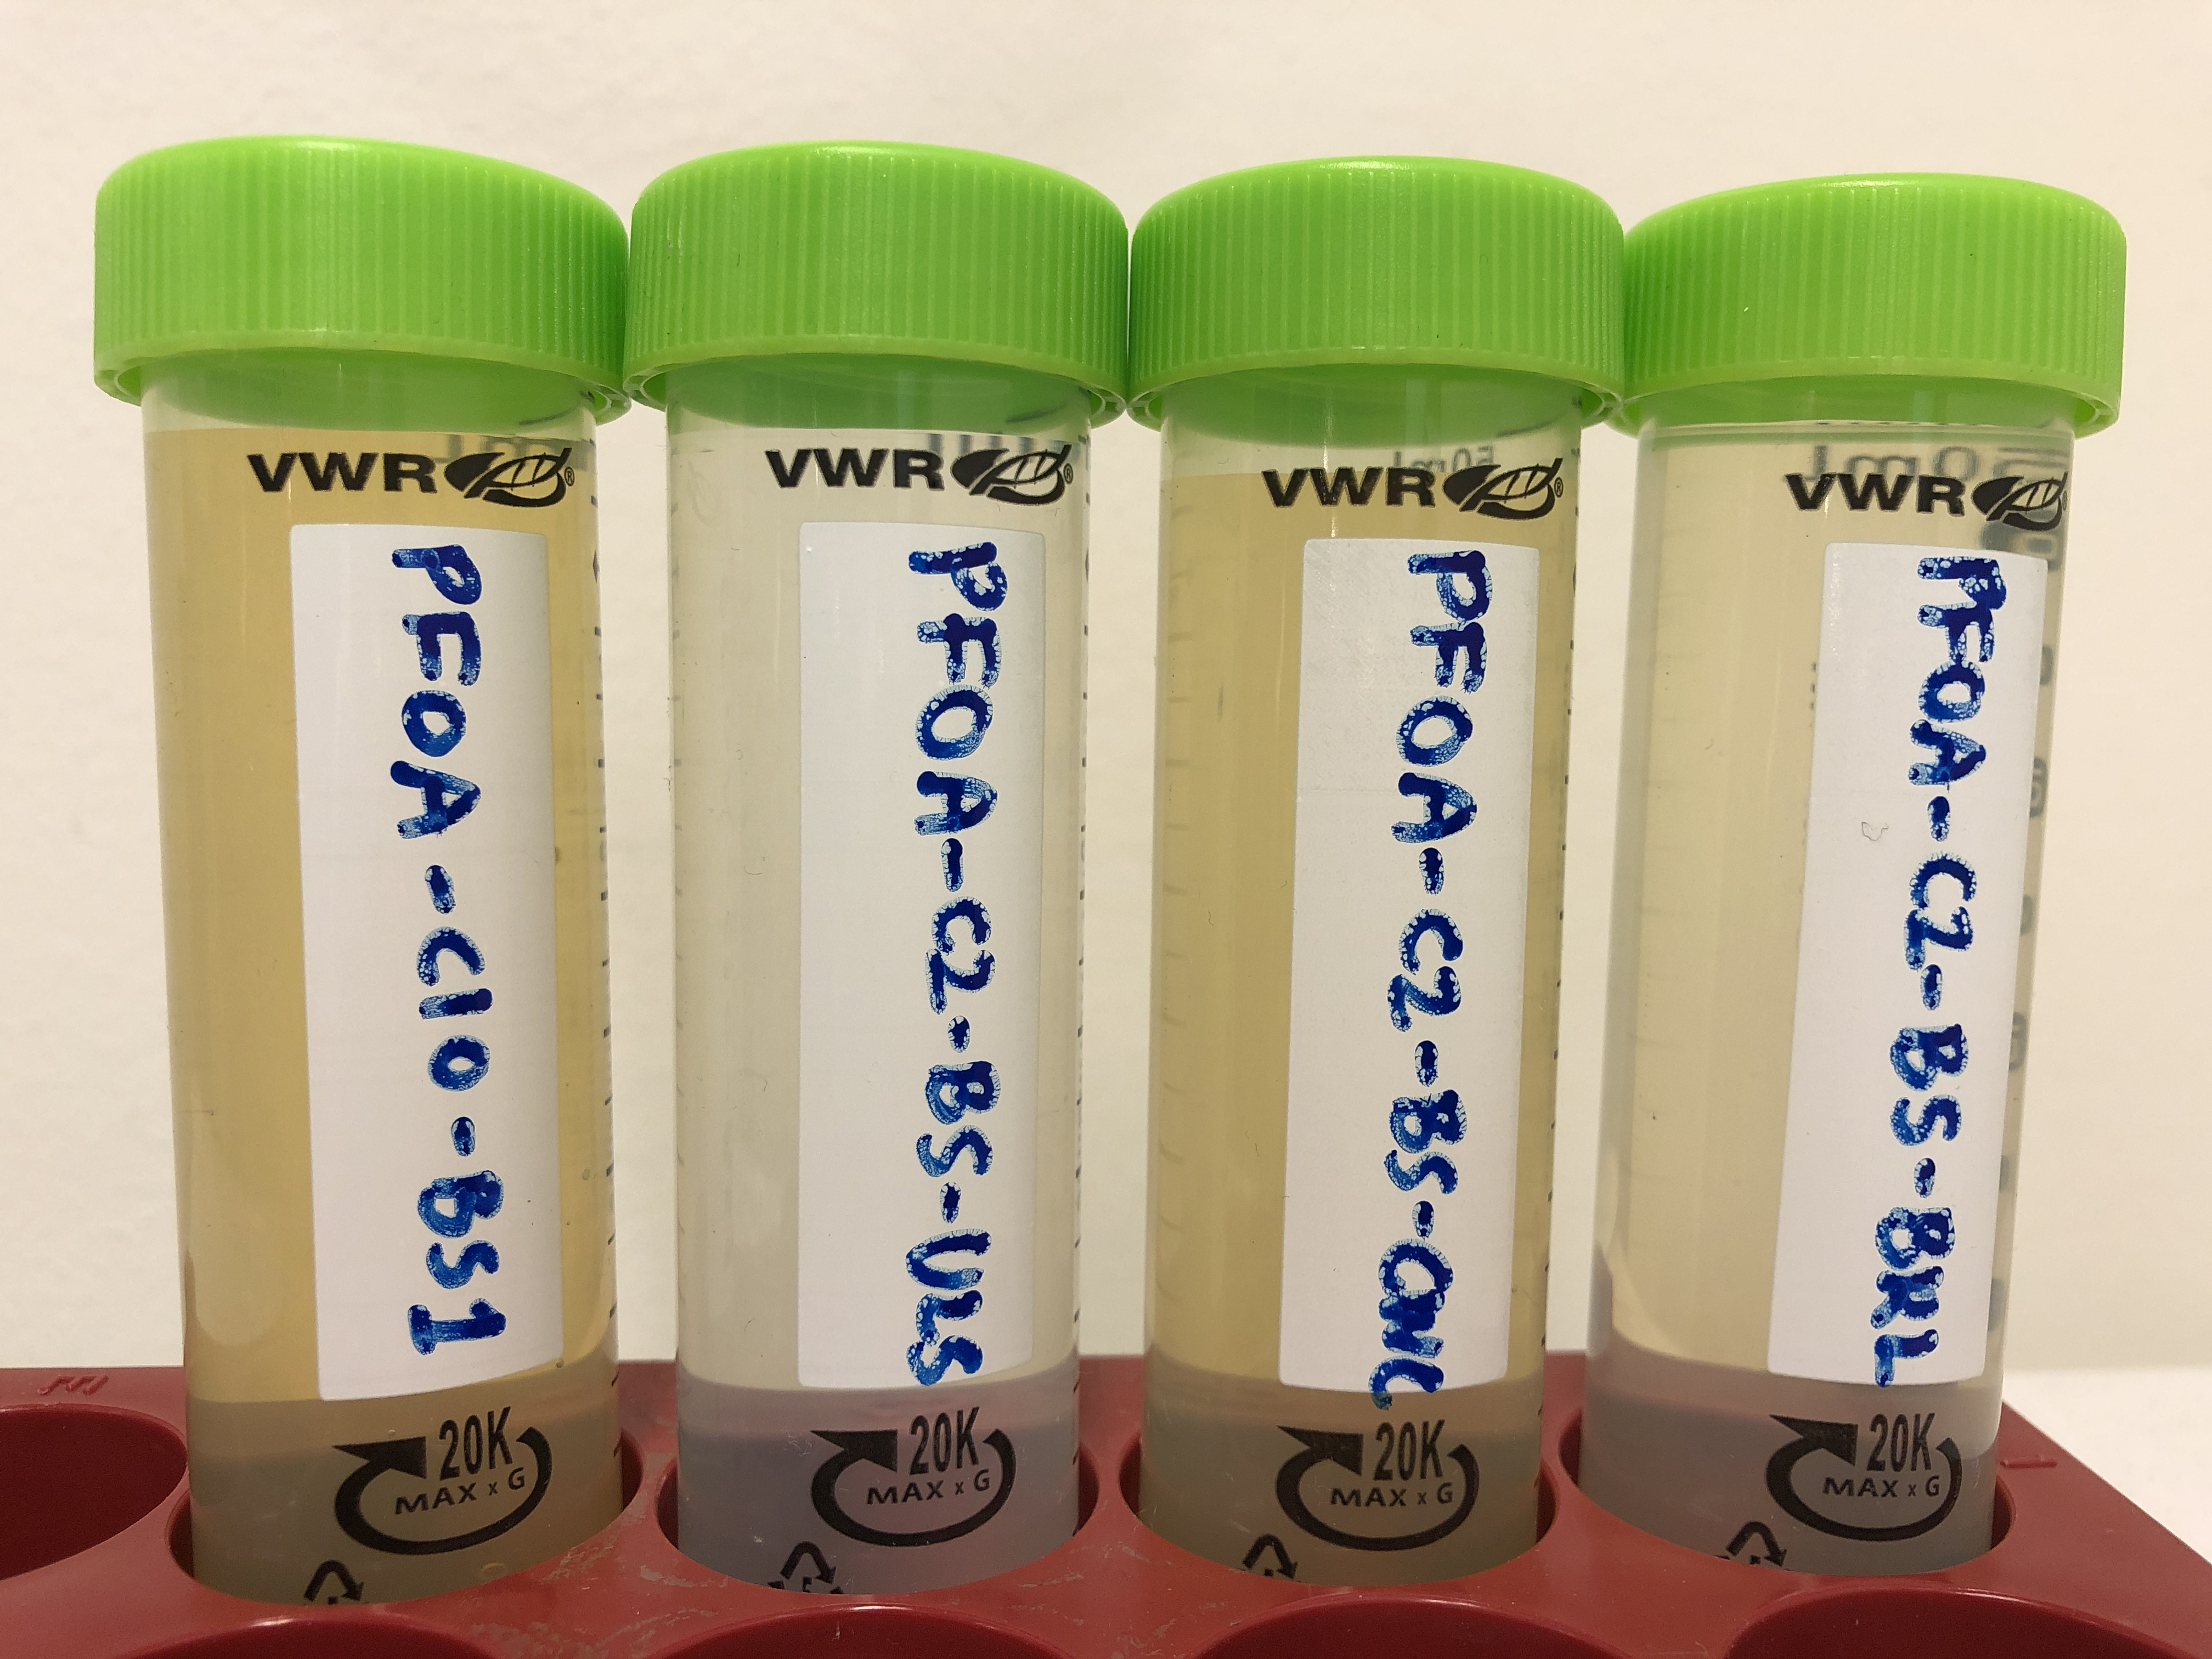
\includegraphics[width=0.45\textwidth]{Bilder/Samples/Filtrate_DOC.JPG}
}
\hfill
\subfloat[\label{subfig:precip}]{%
  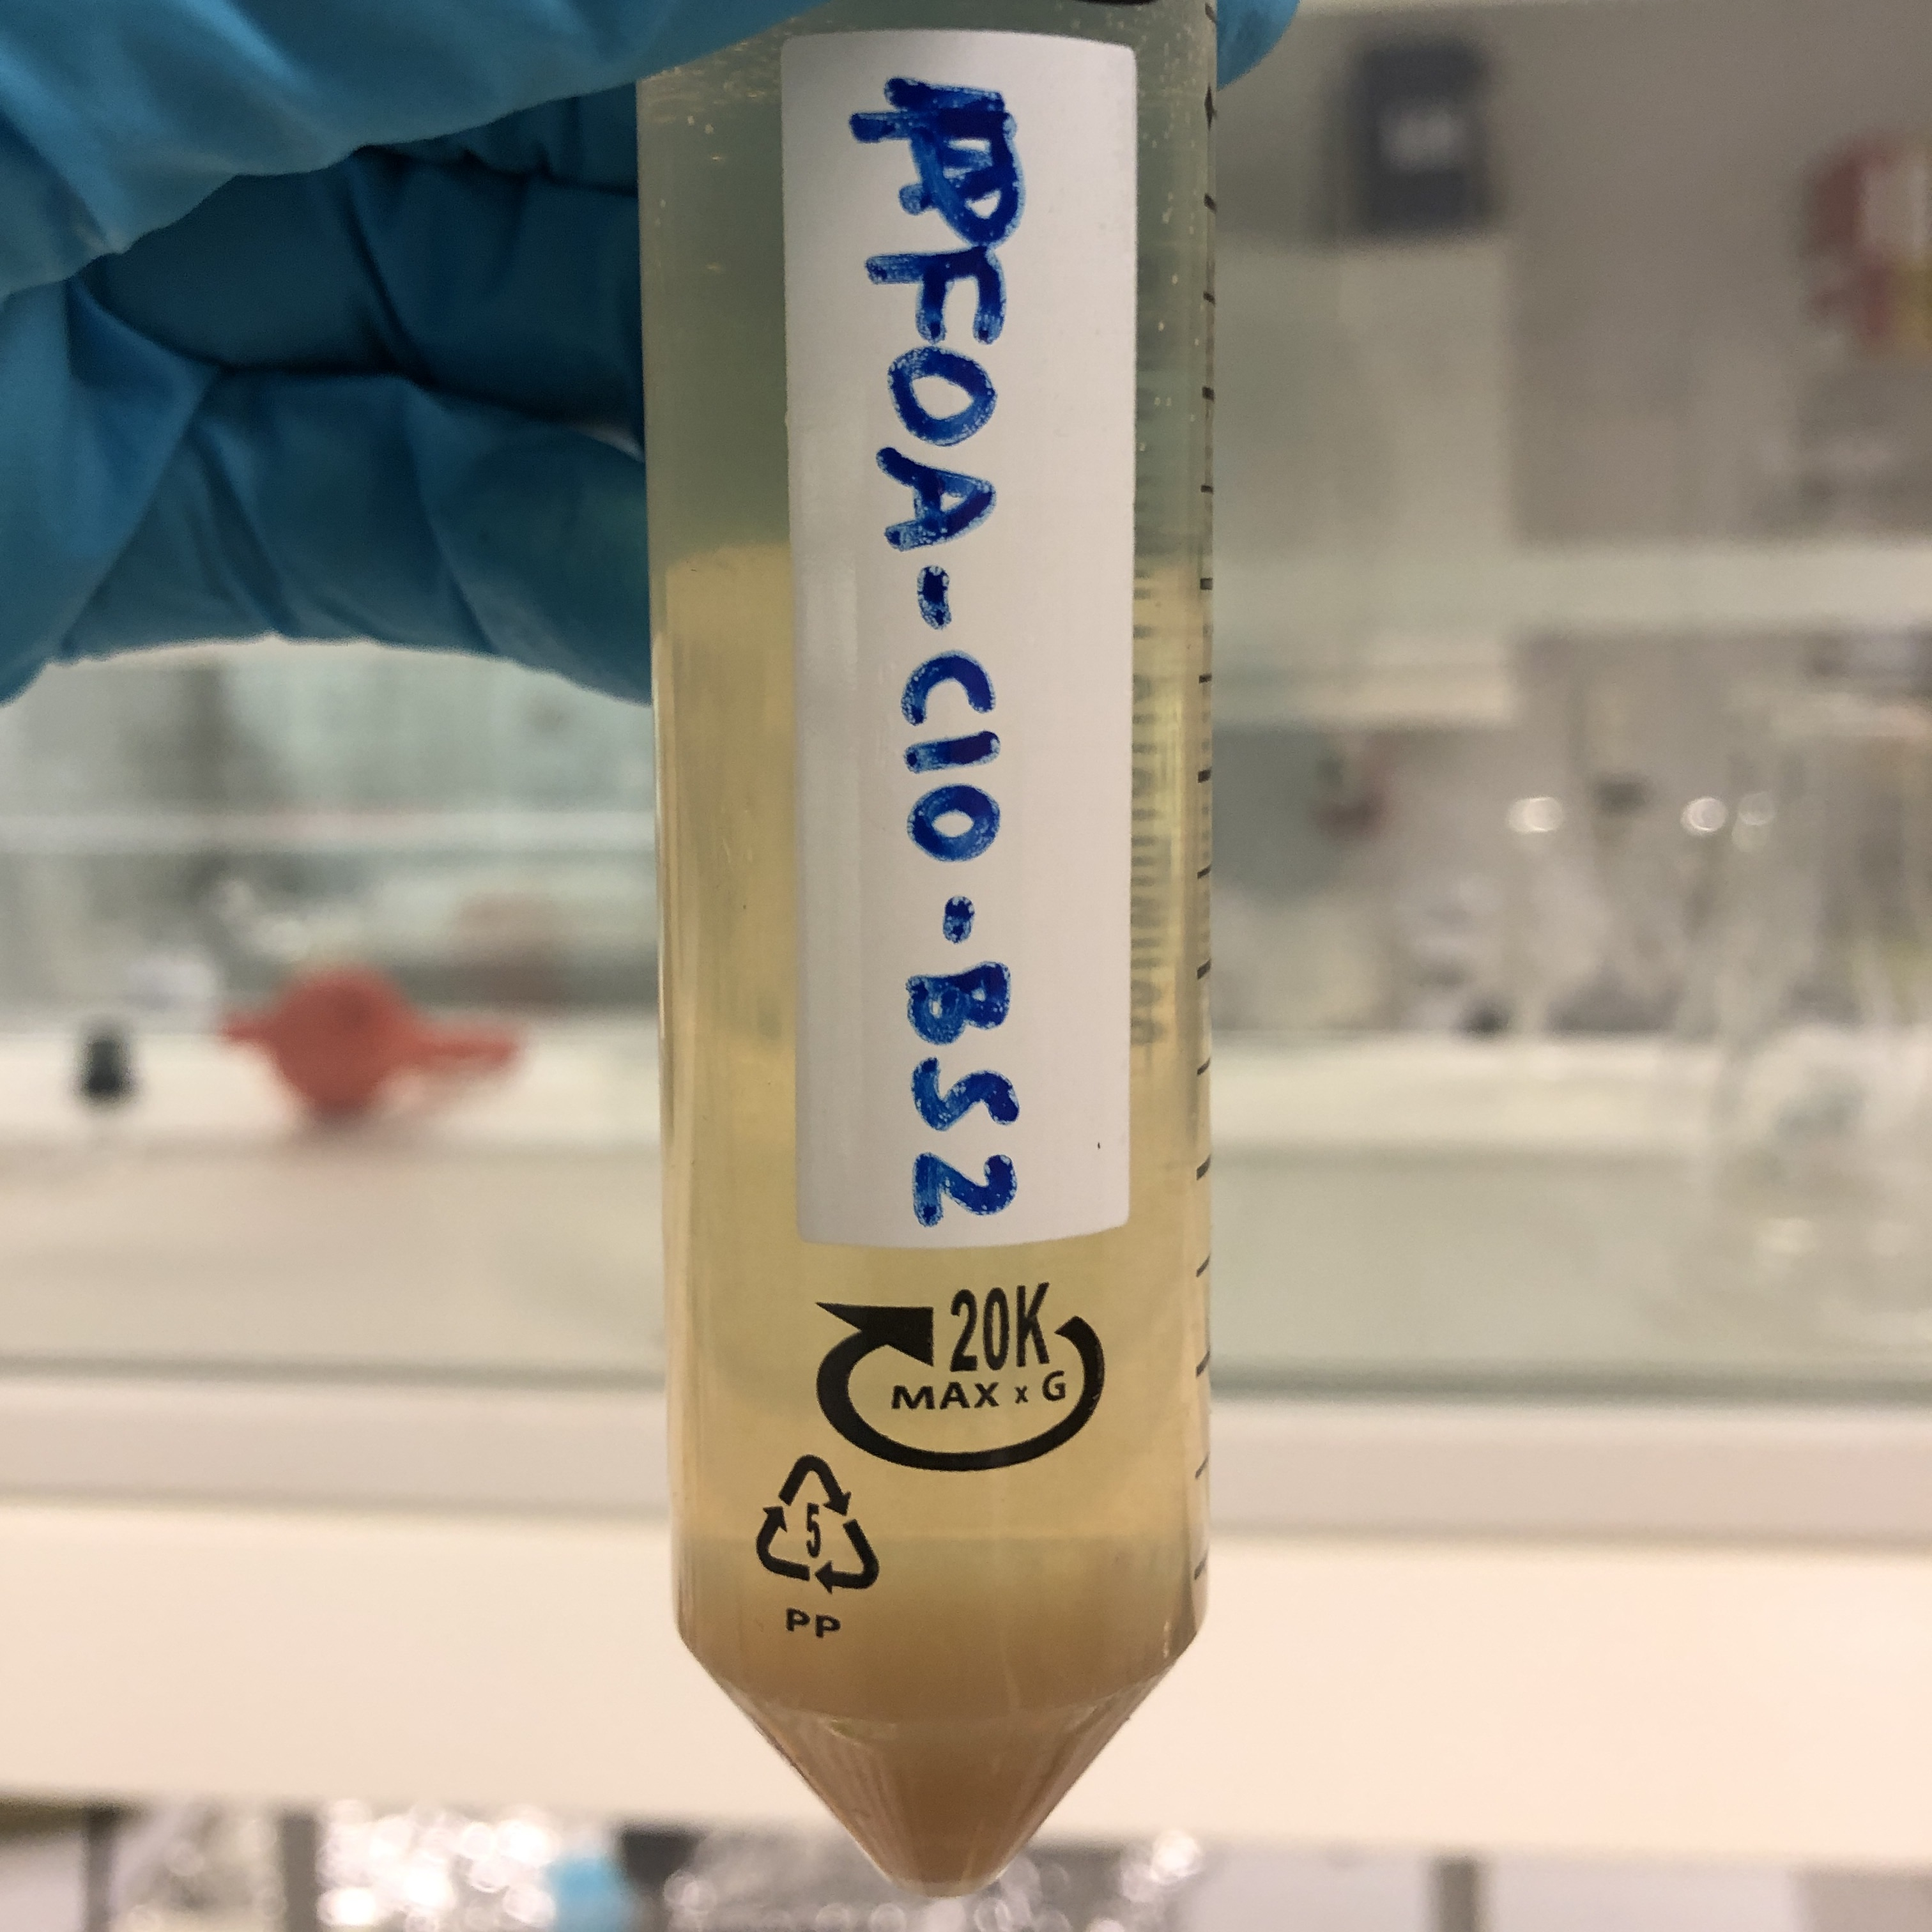
\includegraphics[width=0.45\textwidth]{Bilder/Samples/Precipitation.jpg}
}
\caption{(a) Color of filtrate for each biochar batch test. From left to right: soil only, soil+ULS, soil+CWC, and soil+BRL. (b) Precipitation observed when filtered soil samples were adjusted to pH 3 with 1 M acetic acid.}
\label{fig:DOC_tubes}
\end{figure}


\begin{figure}[htb]
    \centering
    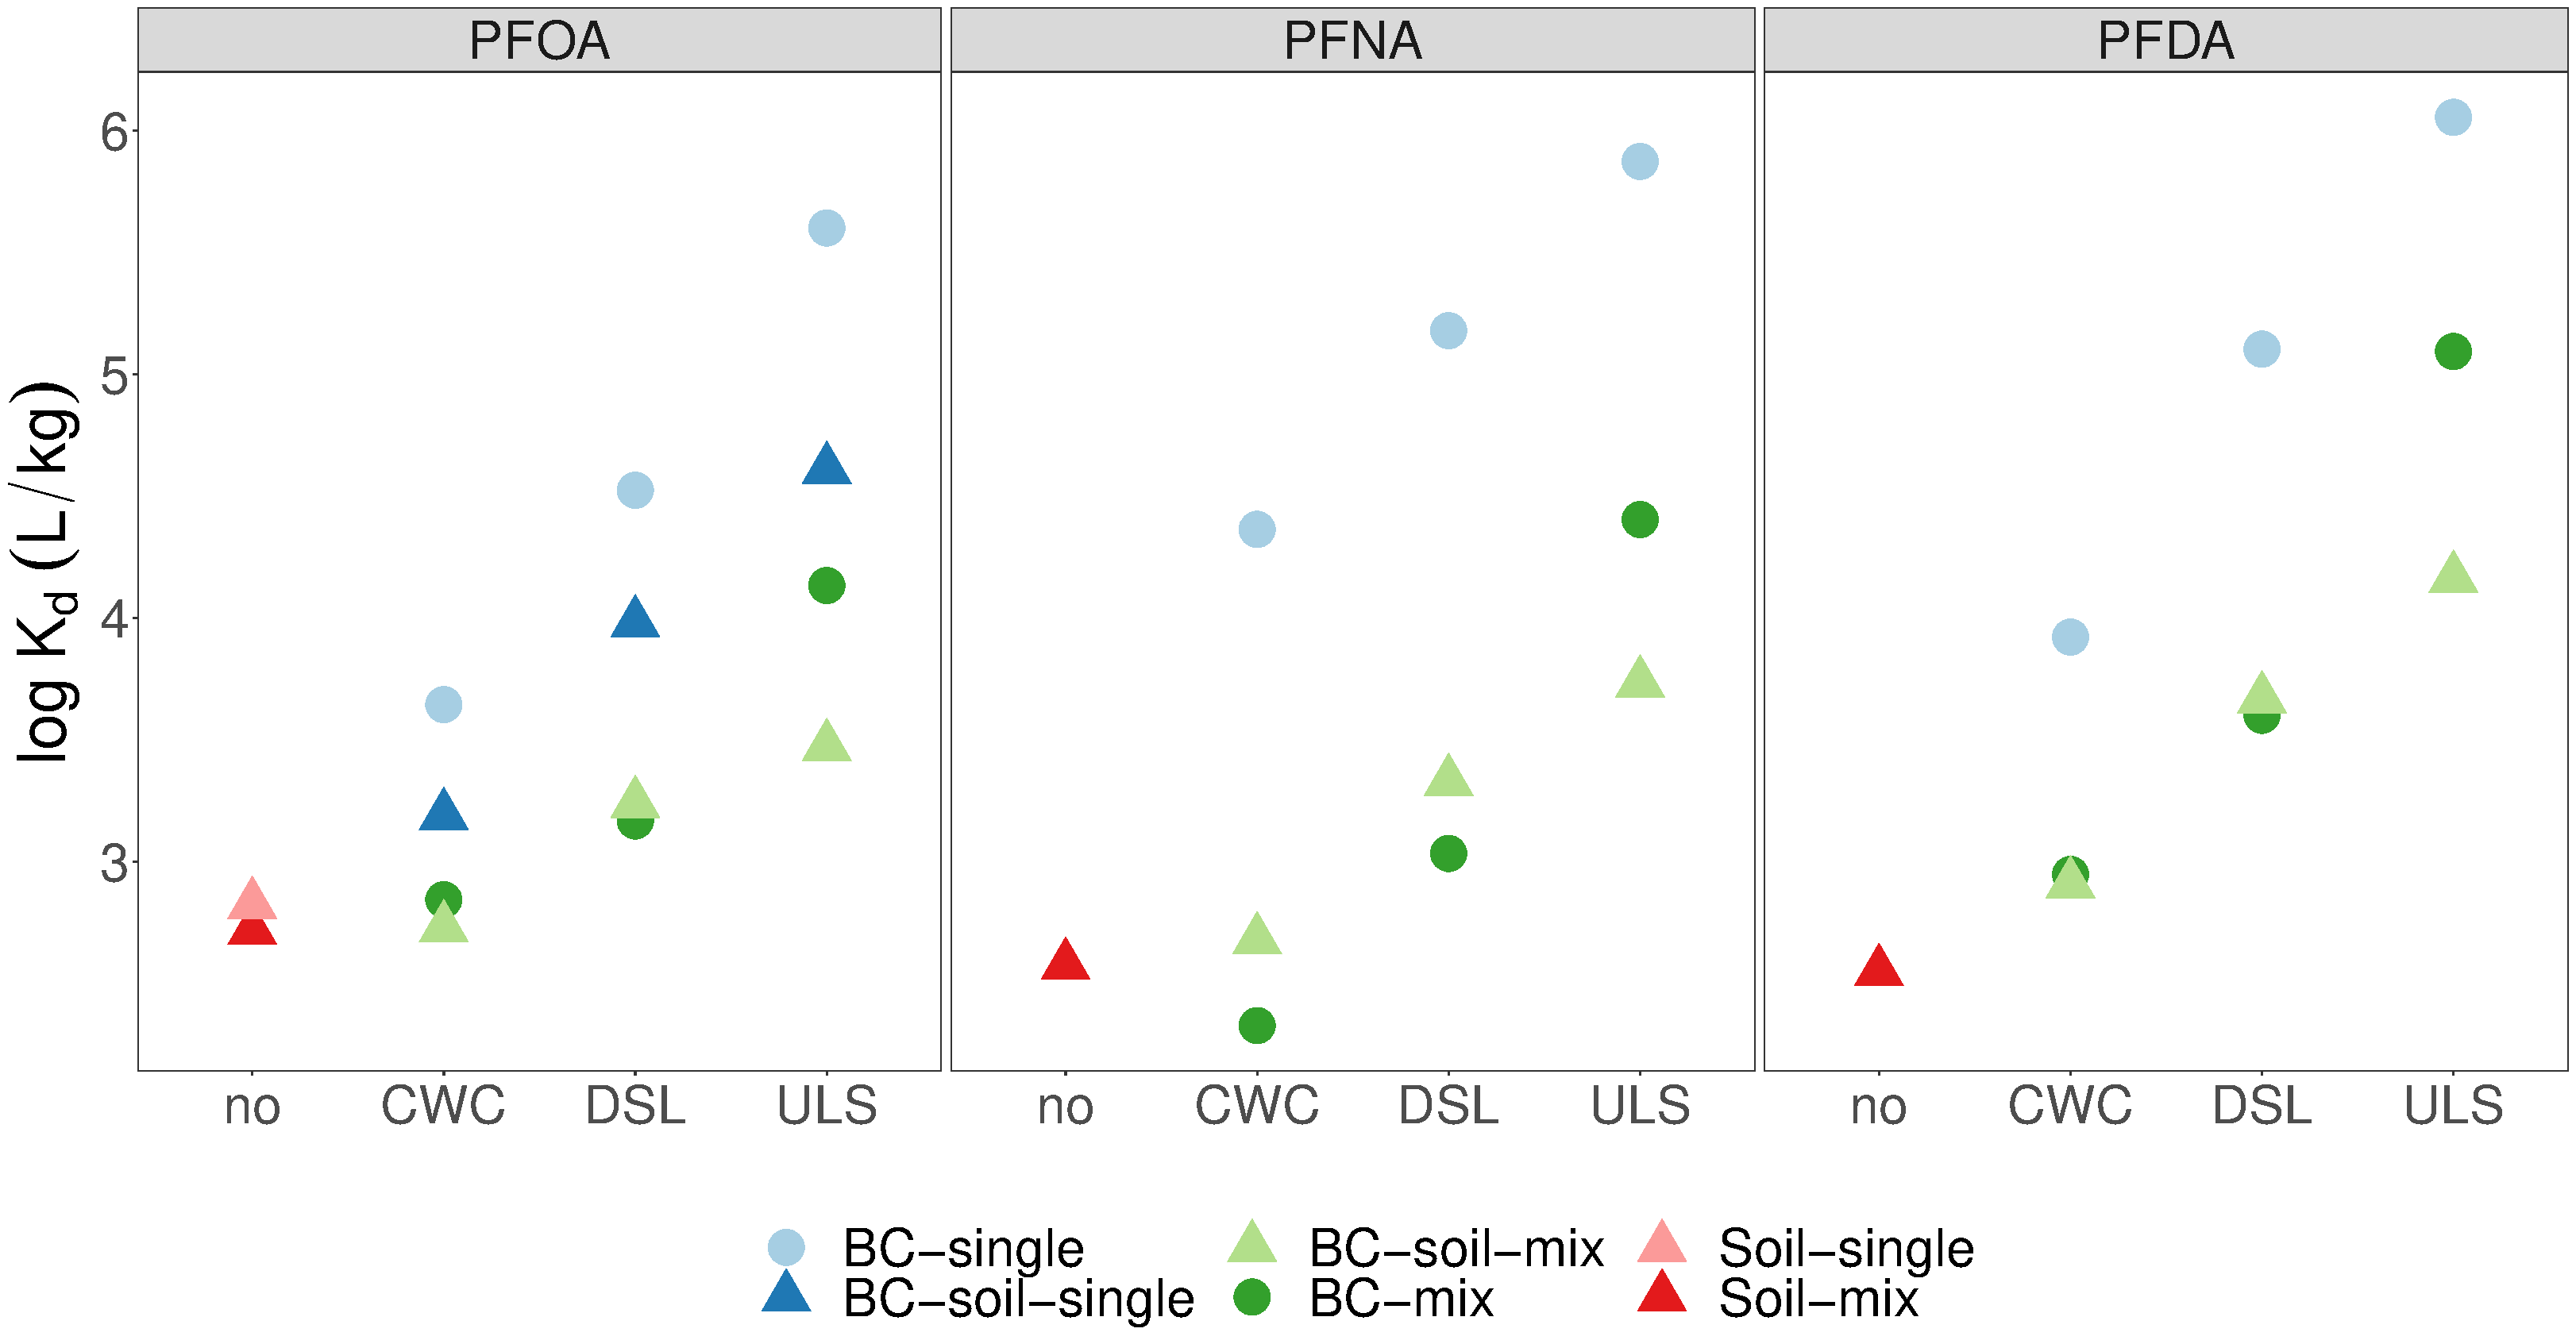
\includegraphics[width=\textwidth]{R/figs/C10.pdf}
    \caption{Sorption attenuation for each TC by soil and/or competing congeners at SC10. The error bars represent the standard deviation of $log~K_d$ for the cocktail batch tests performed in triplicate (not included). The single-compound $log~K_d$'s are single points.}
    \label{fig:C10}
\end{figure}

\begin{figure}[htb]
    \centering
    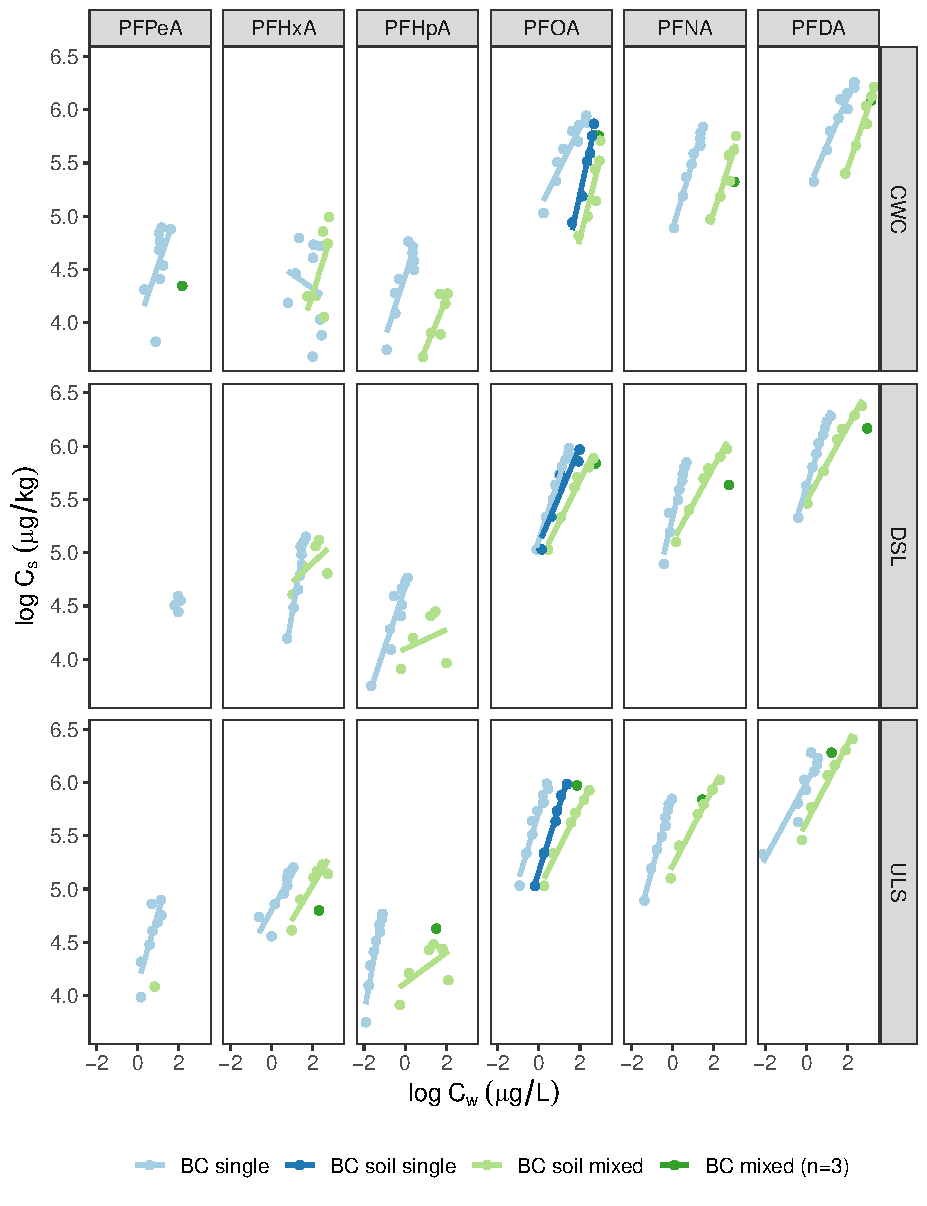
\includegraphics[width=\textwidth]{R/figs/Attenuation.pdf}
    \caption{Sorption attenuation by soil and a cocktail.}
    \label{fig:attenuation}
\end{figure}

\begin{table}
\centering
\caption{Competition factor at SC10 (\cref{tab:spikeConcentrations}) for each compound and biochar. Competition factor is defined as K\textsubscript{d,single}/K\textsubscript{d,mix})$\times$100\%.}
\begin{threeparttable}
\label{tab:competition}
\begin{tabular}{lrrr}
\toprule
 & \multicolumn{3}{c}{Competition factor \%} \\ \cmidrule(l){2-4}
 & CWC & ULS & DSL \\ \midrule
PFPeA & 8.2 & \textsuperscript{*} & \textsuperscript{*} \\
PFHxA & \textsuperscript{*} & 2.3 & \textsuperscript{*} \\
PFHpA & \textsuperscript{*} & 0.2 & \textsuperscript{*} \\
PFOA & 15.8 & 3.4 & 4.4 \\
PFNA & 0.9 & 3.4 & 0.7 \\
PFDA & 10.6 & 10.9 & 3.1 \\ \bottomrule
\end{tabular}
\begin{tablenotes}
\item \textsuperscript{*} Amount in filtrate exceeded the amount spiked due to analytical uncertainty.
\end{tablenotes}
\end{threeparttable}
\end{table}

\subsection{Sorption non-linearity}
$n_F$ is a dimensionless empirical parameter that represents sorption linearity. All isotherms experience sorption site saturation at increasing concentrations indicated by $n_F<1 $ (\cref{tab:summary_stats_single}, which is consistent with the Freundlich model and other studies where sorption to biochar sees $n$-values typically around 0.3-0.7 \citep{Cornelissen2005}. From other studies, $K_F$ increases and $n_F$ decreases with decreasing O/C, H/C, and N/C ratios \citep{Cornelissen2005}. However, this study $K_F$ decreases with decreasing O/C, H/C, and N/C ratios, and no clear trend is seen for $n_F$ \cref{subfig:n}. Meanwhile, it does seem like the nonlinearity coefficients for CWC are more stable with increasing chain lengths than ULS and DSL. Additionally, comparing $n$ across compound isotherms does not make sense due to different spike concentrations being used for each compound. \citep{yin2022insights} suggests that electrostatic interactions between PFCAs and sediment can contribute to further enhancement of saturation of the adsorption sites and that intermolecular electrostatic repulsion between the individual molecules could also result in nonlinear sorption \citep{higgins2006sorption,yin2022insights}.

\citep{yin2022insights} attributes non-linear sorption to three explanations: 1) complex composition of biochar with negative, positive and neutral charges within same matrix, 2) successive saturation of adsorption sites, 3) electrostatic interactions between the PFASs and sediment, 4) electrostatic repulsion from negatively charged carboxylate groups. 

Sorption non-linearity ($n<1$) occurs due to the complex composition of sediment/biochar with both positive and negative charges contributing to either attraction or repulsion, as well as hydrophobic surfaces, and indicates successive saturation of these adsorption sites \citep{yin2022insights}.  

For the short-chain compounds (PFPeA and PFHxA), Correlations are poor which results in higher standard errors and slopes that are unrealistic (PFHxA-DSL: n=1.11 and PFHpA-ULS: 1.08). Possible explanations for the poor correlations for PFPeA and PFHxA are poor biochar affinity, but the standard error is also large so that the isotherm may actually be linear ($\pm$ 0.11 for both). For PFPeA- and PFHxA-CWC, it appears that CWC sorption sites have been saturated since most points center around the same area, which means that CWC reaches sorption maximum at $~$4000 $\mu g~kg^{-1}$. However, four points are insufficient to conclude that CWC has the lowest affinity and capacity to sorb short-chain PFCAs. The CWC isotherms had the widest concentration intervals for $C_w$, which can be explained by CWC being the weakest sorbent of the three biochars studied, resulting in higher aqueous concentrations than for the sludge biochars. 

\subsubsection{Isotherm concentration range}
ULS and DSL gave isotherms typically across 0-1.5 orders of magnitude, which indicates that either higher spike concentrations or a lower BC dosage should have been used for the batch tests and that the sludge biochars have a higher sorptive capacity compared with CWC. The batch tests were spiked at 10 concentrations over four orders of magnitude where the lowest concentration was aimed at being close to the instrumental LOQ. Poor signals were achieved for the SC1 points and were removed from the data analysis to improve the certainty of the regression analysis. By doing this the spike concentration interval was reduced to two orders of magnitude \cref{tab:spikeConcentrations}. The concentration range achieved was an average of 1.3 log units for the batch test filtrate, in contrast to the desired concentration range over 4 log units. In retrospect, spike concentrations at each log unit should have been selected instead of spreading the ten concentrations evenly across the concentration range. Gaining valid points across a wider concentration range could affect the $n_F$-value acheived. 

%%%%%%%%%%%%%%%%%%%%%%%%%%%%%%%%%%%%%%%%%%%%%%%%%%%%%%%%%%%%%%%%%%%%%%%%%%%%%%%%%%%%%%%%%%%%%%%%%%%%%%%%%%%%%%%%%%%%%%%%%%%%%%%%%%%%%%%%%%%%%%%%%%%%%%%%%%%%%%%%%%%%%%%%%%%%%%%%%%%%%%%%%%%%%%%%%%%%%%%%%%%%%%%%%%%%%%%%%%%%%%%%%%%%%%%%%%%%%%%%%%%%%%%%%%%%%%%%%%%%%%%%%%%%%%%%%%%%%%%%%%%%%%%%%%%%%%%%%%%%%%%%%%%%%%%%%%%%%%%%%%%%%%%%%%%%%%%%%%%%%%%%%%%%%%%%%%%%%%%%%%%%%%%%%%%%%%%%%%%%%%%%%%%%%%%%%%%%%%%%%%%%%%%%%%%%%%%%%%%%%%%%%%%%%%%%%%%%%%%%%%%%%%%%%%%%%%%%%%%%%%%%%%%%%%%%%%%%%%%%%%%%%%%%%%%%%%%%%%%%%%%%%%%%%%%%%%%%%%%%%%%%%%%%%%%%%%%%%%%%%%%%

\section{Effect of biochar properties on sorption}
This section compares the distribution coefficients derived for ULS, DSL and CWC to biochar composition of main elements (C, H, O, N), trace elements (Ca and Fe), and surface area (SA) and pore volume (PV) in order to gain insights into possible sorption mechanisms. In the comparison between sorbent properties and sorption coefficients for each biochar type, PFOA, PFNA and PFDA have been used because they gave the best sorption isotherms. $log~K_F$ has been normalized to 1 $\mu g~L^{-1}$ which is used as the distribution coefficients in this discussion.

\subsection{Surface area and pore volume}

\begin{table}
\centering
\caption{Surface area (SA), pore volume (PV), elemental content (C, O, H, N) and ratios for the biochars produced for the batch tests.}
\adjustbox{max width=\textwidth}{
\label{tab:SAPV}
\begin{tabular}{llrrrrrrlllllll}
\toprule
Biochar & Pyrolysis & \multicolumn{3}{l}{N\textsubscript{2} sorption} & \multicolumn{3}{l}{CO\textsubscript{2} sorption} & \multicolumn{4}{c}{Elemental content} & \multicolumn{3}{c}{Elemental ratio} \\
sorbent & temperature & \multicolumn{3}{l}{(pores \textgreater 1.5 nm)} & \multicolumn{3}{l}{(pores 0.4-1.5 nm)} & & & & & & & \\ \cmidrule(l){3-5} \cmidrule(l){6-8} \cmidrule(l){9-12} \cmidrule(l){13-15} & (\textdegree C) & BET SA  & BJH PV & log SA/PV & DFT SA & DFT PV & log SA/PV & C & O & H & N & O/C & H/C & N/C \\
& & ($\mathrm{m^2~g^{-1}}$) & (cm\textsuperscript{3} g\textsuperscript{-1}) & ($\mathrm{m^2 cm^{-3}}$) & ($\mathrm{m^2~g^{-1}}$) & (cm\textsuperscript{3} g\textsuperscript{-1}) & ($\mathrm{m^2 cm^{-3}}$) & (\%) & (\%) & (\%) & (\%) & & & \\ \midrule
CWC & 700 & 323 & 0.017 & 3.21 & 683 & 0.186 & 3.54 & 91.4 & 5.50 & 1.01 & 0.69 & 0.06 & 0.01 & 0.008       \\
ULS & 700 & 128 & 0.126 & 2.80 & 165 & 0.047 & 3.57 & 29.6 & 57.1 & 1.24 & 1.13 & 1.9  & 0.04 & 0.04        \\
DSL & 700 & 110 & 0.111 & 2.80 & 87  & 0.027 & 3.51 & 13.5 & 61.4 & 1.05 & 0.82 & 4.6  & 0.08 & 0.06       \\ \bottomrule
\end{tabular}}
\end{table}

\subsubsection{Pore size distribution of small pores}
\cref{tab:SAPV} shows the total surface area (SA, m\textsuperscript{2}/g) and pore volume (PV, cm\textsuperscript{3}/g) for the three biochars used in the sorption experiments in this study. For small pores (0.4-1.5 nm, CO\textsubscript{2} sorptiometry), SA of CWC was $\sim$six times higher than ULS and DSL (165 and 87  m\textsuperscript{2} g\textsuperscript{-1}, respectively), and PV also followed the same order. Previous research agree that large internal surface area and pore volume are desirable for strong sorption of organic contaminants because it increases available sorption sites \citep{ahmed2020per,Hale2016}. The high SA and PV of CWC suggests that this biochar has the highest fraction of available sorption sites compared to ULS and DSL within the micropore range ($\le$ 2 nm). However, as graphed in \cref{fig:PZD_small}a-c, it becomes becomes evident that nearly 80\% of the SA and 60\% of the PV of CWC is located in nanopores $<$ 0.6 nm. These pores become nearly inaccessible to the adsorbate molecules because the perfluorinated chains are quite large and rigid, preventing them from entering pores that are too small, and if managing to enter, they have difficulties adapting its shape to the pore wall to sorb strongly due to steric hindrance. Additionally, molecular size increases with chain length, which makes it even more difficult for long-chain PFASs to diffuse into the smallest pores. 

\cref{tab:molecsize} lists effective cross-sectional diameter ($D_{eff}$) and maximum diameter ($D_{max}$) of each TC (the definitions of $D_{eff}$ and $D_{max}$ are illustrated in \cref{fig:molecularSize}). PFCAs C5-C10 range from 0.45-0.72 nm $D_{eff}$ and 0.96-1.54 nm $D_{max}$. Maximum sorption is acheived when the molecular dimensions of the PFAS congeners match the pore size and shape \citep{Hale2016}. Since the PZD within the CO\textsubscript{2}-range is dominated by pores $<$0.6 nm for CWC, ULS, and DSL, sorption of PFPeA, PFHxA, and PFHpA is only possible if the congeners enter the pores at the exact right angle, whereas PFOA, PFNA, and PFDA will experience size exclusion, and the pores are easily blocked by large molecules. Therefore, sorption of PFAS in the CO\textsubscript{2}-range is insignificant and cannot explain the differences in $log~K_F$ between biochar types, especially since strongest sorption was measured for long-chain PFCAs (PFOA, PFNA, and PFDA).

%consider removing log SA/PV graph, and rather wait with this discussion for the large pores. There are only minor differences in SA/PV ratio between the biochars (cumulative ratios: 3 674, 3 502, and 3 206 m\textsuperscript{2} cm\textsuperscript{-3} for CWC, ULS, and DSL respectively), which means that despite CWC being far more numerous in nanopores than ULS and DSL, the structure of these pores are similar, and the highest proportion of nanopores for all three biochars are $<$0.6 nm.

\begin{figure}[htb]
    \centering
    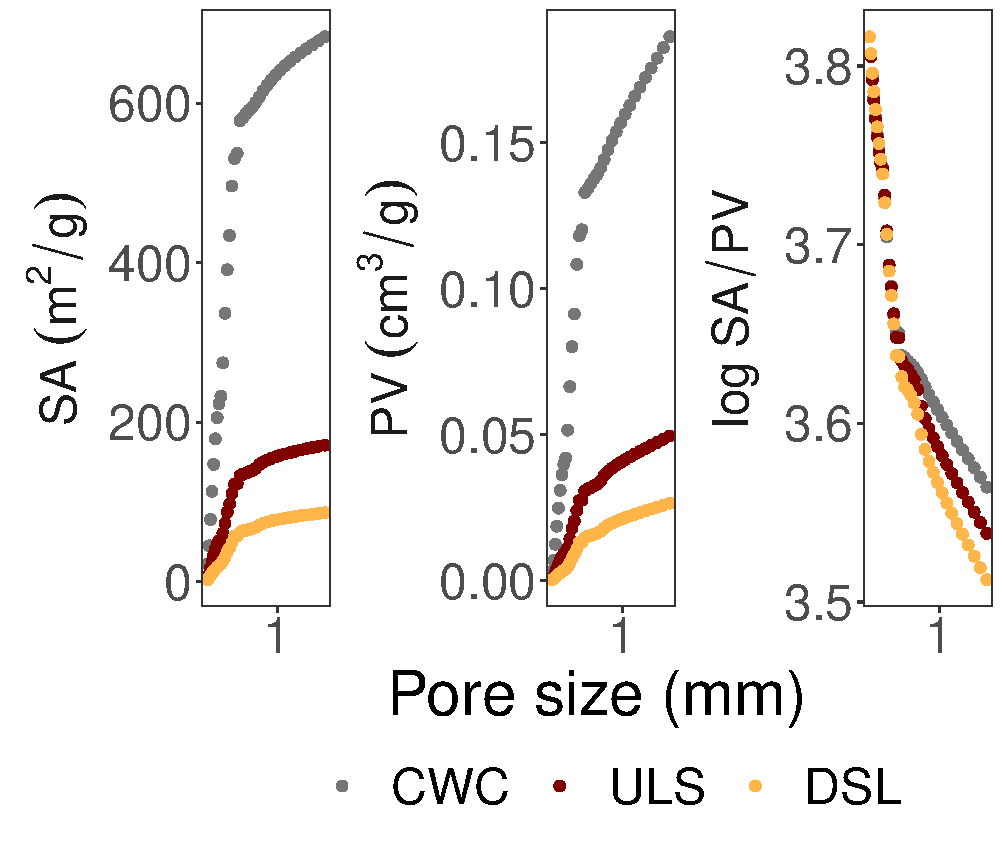
\includegraphics[width=\textwidth]{R/figs/PZD_SAPV_C_small_plot.pdf}
    \caption{Cumulative pore size distribution for pores 0.4-1.5 nm using DFT.}
    \label{fig:PZD_small}
\end{figure}

\begin{table}
\caption{Effective cross-sectional diameter ($D_{eff}$) and maximum diameter ($D_{max}$) of TCs interpolated and extrapolated by linear regression from calculations performed by \cite{inoue2012size} on PFOA and other PFCAs with chain lengths 11-18.}
\centering
\begin{threeparttable}
\label{tab:molecsize}
\begin{tabular}{llll}
\toprule
Compound & CF\textsubscript{2} & $D_{eff}$ & $D_{max}$ \\ 
& chain & (nm) & (nm) \\ \midrule
PFPeA & 5  & 0.45  & 0.96  \\
PFHxA & 6  & 0.50  & 1.08  \\
PFHpA & 7  & 0.56  & 1.19  \\
PFOA\textsuperscript{*} & 8 & 0.61 & 1.36 \\
PFNA & 9 & 0.67 & 1.42  \\
PFDA & 10 & 0.72 & 1.54  \\ \bottomrule                                    
\end{tabular}
\begin{tablenotes}
\item \textsuperscript{*} Value from \cite{inoue2012size}
\end{tablenotes}
\end{threeparttable}
\end{table}

\begin{figure}
    \centering
    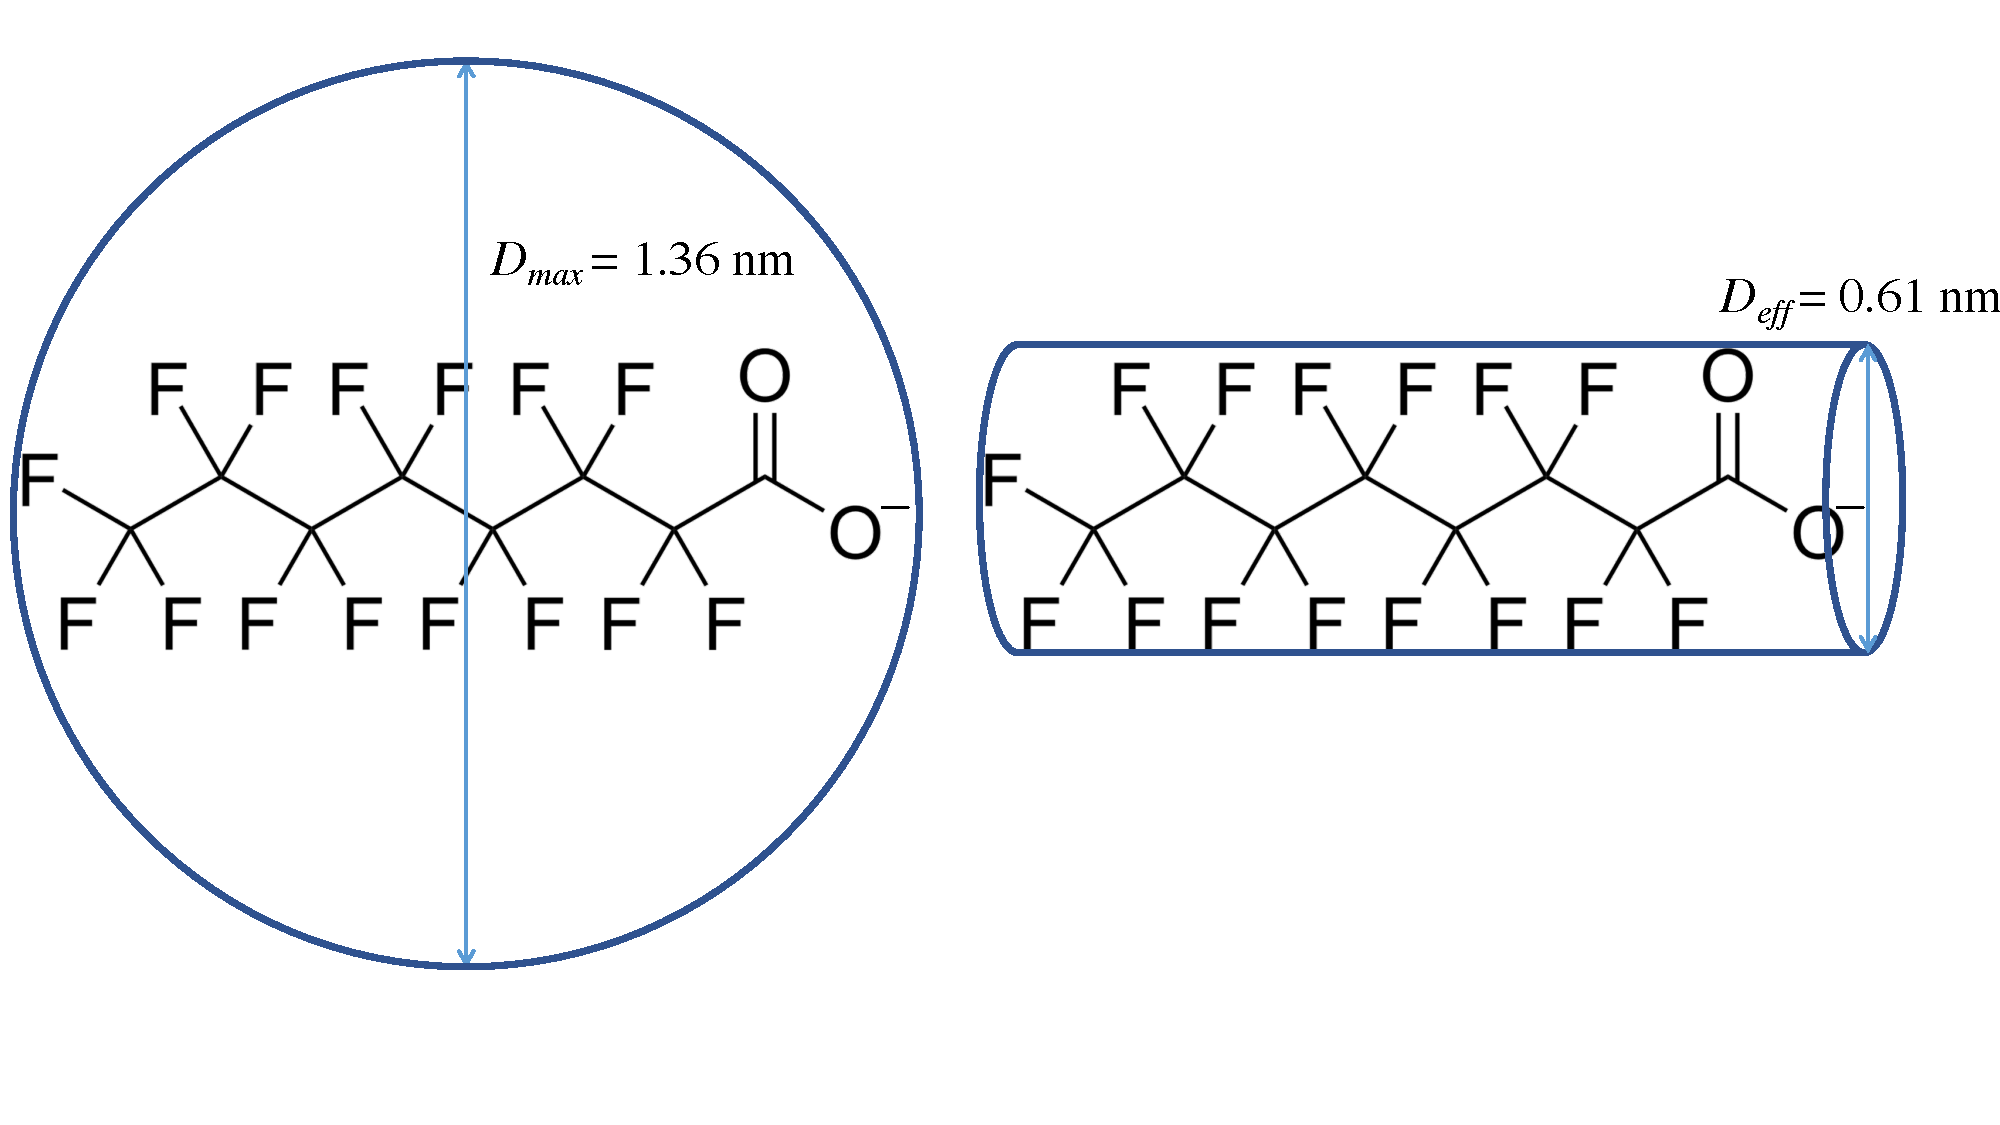
\includegraphics[width=0.8\textwidth, trim={0 2cm 0 0},clip]{Diagrams/Molecular_size.pdf}
    \caption{Definition of effective cross-sectional diameter ($D_{eff}$) and maximum diameter ($D_{max}$) shown for PFOA.}
    \label{fig:molecularSize}
\end{figure}

\subsubsection{Pore size distribution of large pores}
Similar to the trend for small pores, CWC also had the largest cumulative SA for pores $>$1.5 nm (323 m\textsuperscript{2} g\textsuperscript{-1}) versus 110 and 128 m\textsuperscript{2} g\textsuperscript{-1} for DSL and ULS, respectively. \cref{fig:PZD_large}a shows that the highest proportion of SA is allocated to pores between 1.5-5 nm for all three biochar samples. ULS had the highest cumulative PV (0.126 cm\textsuperscript{3} g\textsuperscript{-1}), whereas PV for CWC was one order of magnitude lower (0.017 cm\textsuperscript{3} g\textsuperscript{-1}). Further, the development of PV with pore size in \cref{fig:PZD_large}b shows a clear distinction between CWC and the two sewage sludge biochars. CWC has most of its PV in pores $<$3 nm, whereas ULS and DSL have volumes that increase steadily up to the maximum pore size of 35 nm. This difference becomes important when interpreting a new parameter, the SA/PV ratio, which is graphed in \cref{fig:PZD_large}c. The SA/PV better indicates the spatial arrangement of pores, where a low ratio reflects pores of maximum sorption volume. Here, ULS and DSL have low and equivalent log SA/PV ratios of 2.8 compared to CWC, which has a higher ratio of 3.21 (\cref{tab:SAPV}). Previous studies are consistent in concluding that a large internal surface area and pore volume of adsorbents is one of the most important parameters achieving high sorption capacity of PFAS \citep{du2014adsorption,Sormo2021,Hale2016,ahmed2020per}. Likewise, the results from this study provides clear indications that a low SA/PV ratio can be used to explain higher sorption capacity of ULS and DSL. Since the pores of CWC consists almost exclusively of pores $<$3 nm, whereas ULS and DSL have pores of larger size, this is the most plausible explanation for why CWC is the weakest sorbent among the three samples in this study. The shift observed by comparing SA and PV together demonstrates the importance of considering both pore size \textit{and} surface area when evaluating available sorption sites on biochar.

Since ULS and DSL have nearly equivalent SA/PV ratios, another parameter is needed to explain why ULS is a better sorbent than DSL in this study (\cref{fig:PZD_large}c). Apart from SA and PV, carbon content has shown to be a good predictor of sorption affinity to PFAS from previous literature \citep{Hale2016}. A clear distinction in pore structure emerges by by normalizing the SA/PV ratio for C-content, whereby ULS consists of 29.6 \% C versus 13.5 \% for DSL (\cref{fig:PZD_large}d). ULS has a lower (SA/PV)/C ratio (CALCULATE!!), which means that the pore walls of ULS consists of a higher percentage C making the pore walls more hydrophobic and enhances sorption affinity of PFAS. 

\cref{fig:Kd_SAPV_C} also shows that individually, C and SA/PV does not explain sorption, but together they do.  

In summary, difference in sorption between CWC, DSL, and ULS can be explained by 1) difference in nanopore and micropore structure, where a higher number of large micropores signified by low SA/PV ratio is more ideal for sorption of long-chain PFASs such as PFOA, PFNA, and PFDA, and 2) a higher proportion of carbon in the pore wall matrix further enhances sorption by creating more hydrophobic sorption surfaces. Since the conclusions drawn for the sorption mechanisms contributing to PFCA sorption is based on only three biochar samples, further research within this area should test if a higher sample size comply with the suggestion that pore size size and structure is the most important determinant for sorption of organic contaminants. 

\begin{figure}[htb]
    \centering
    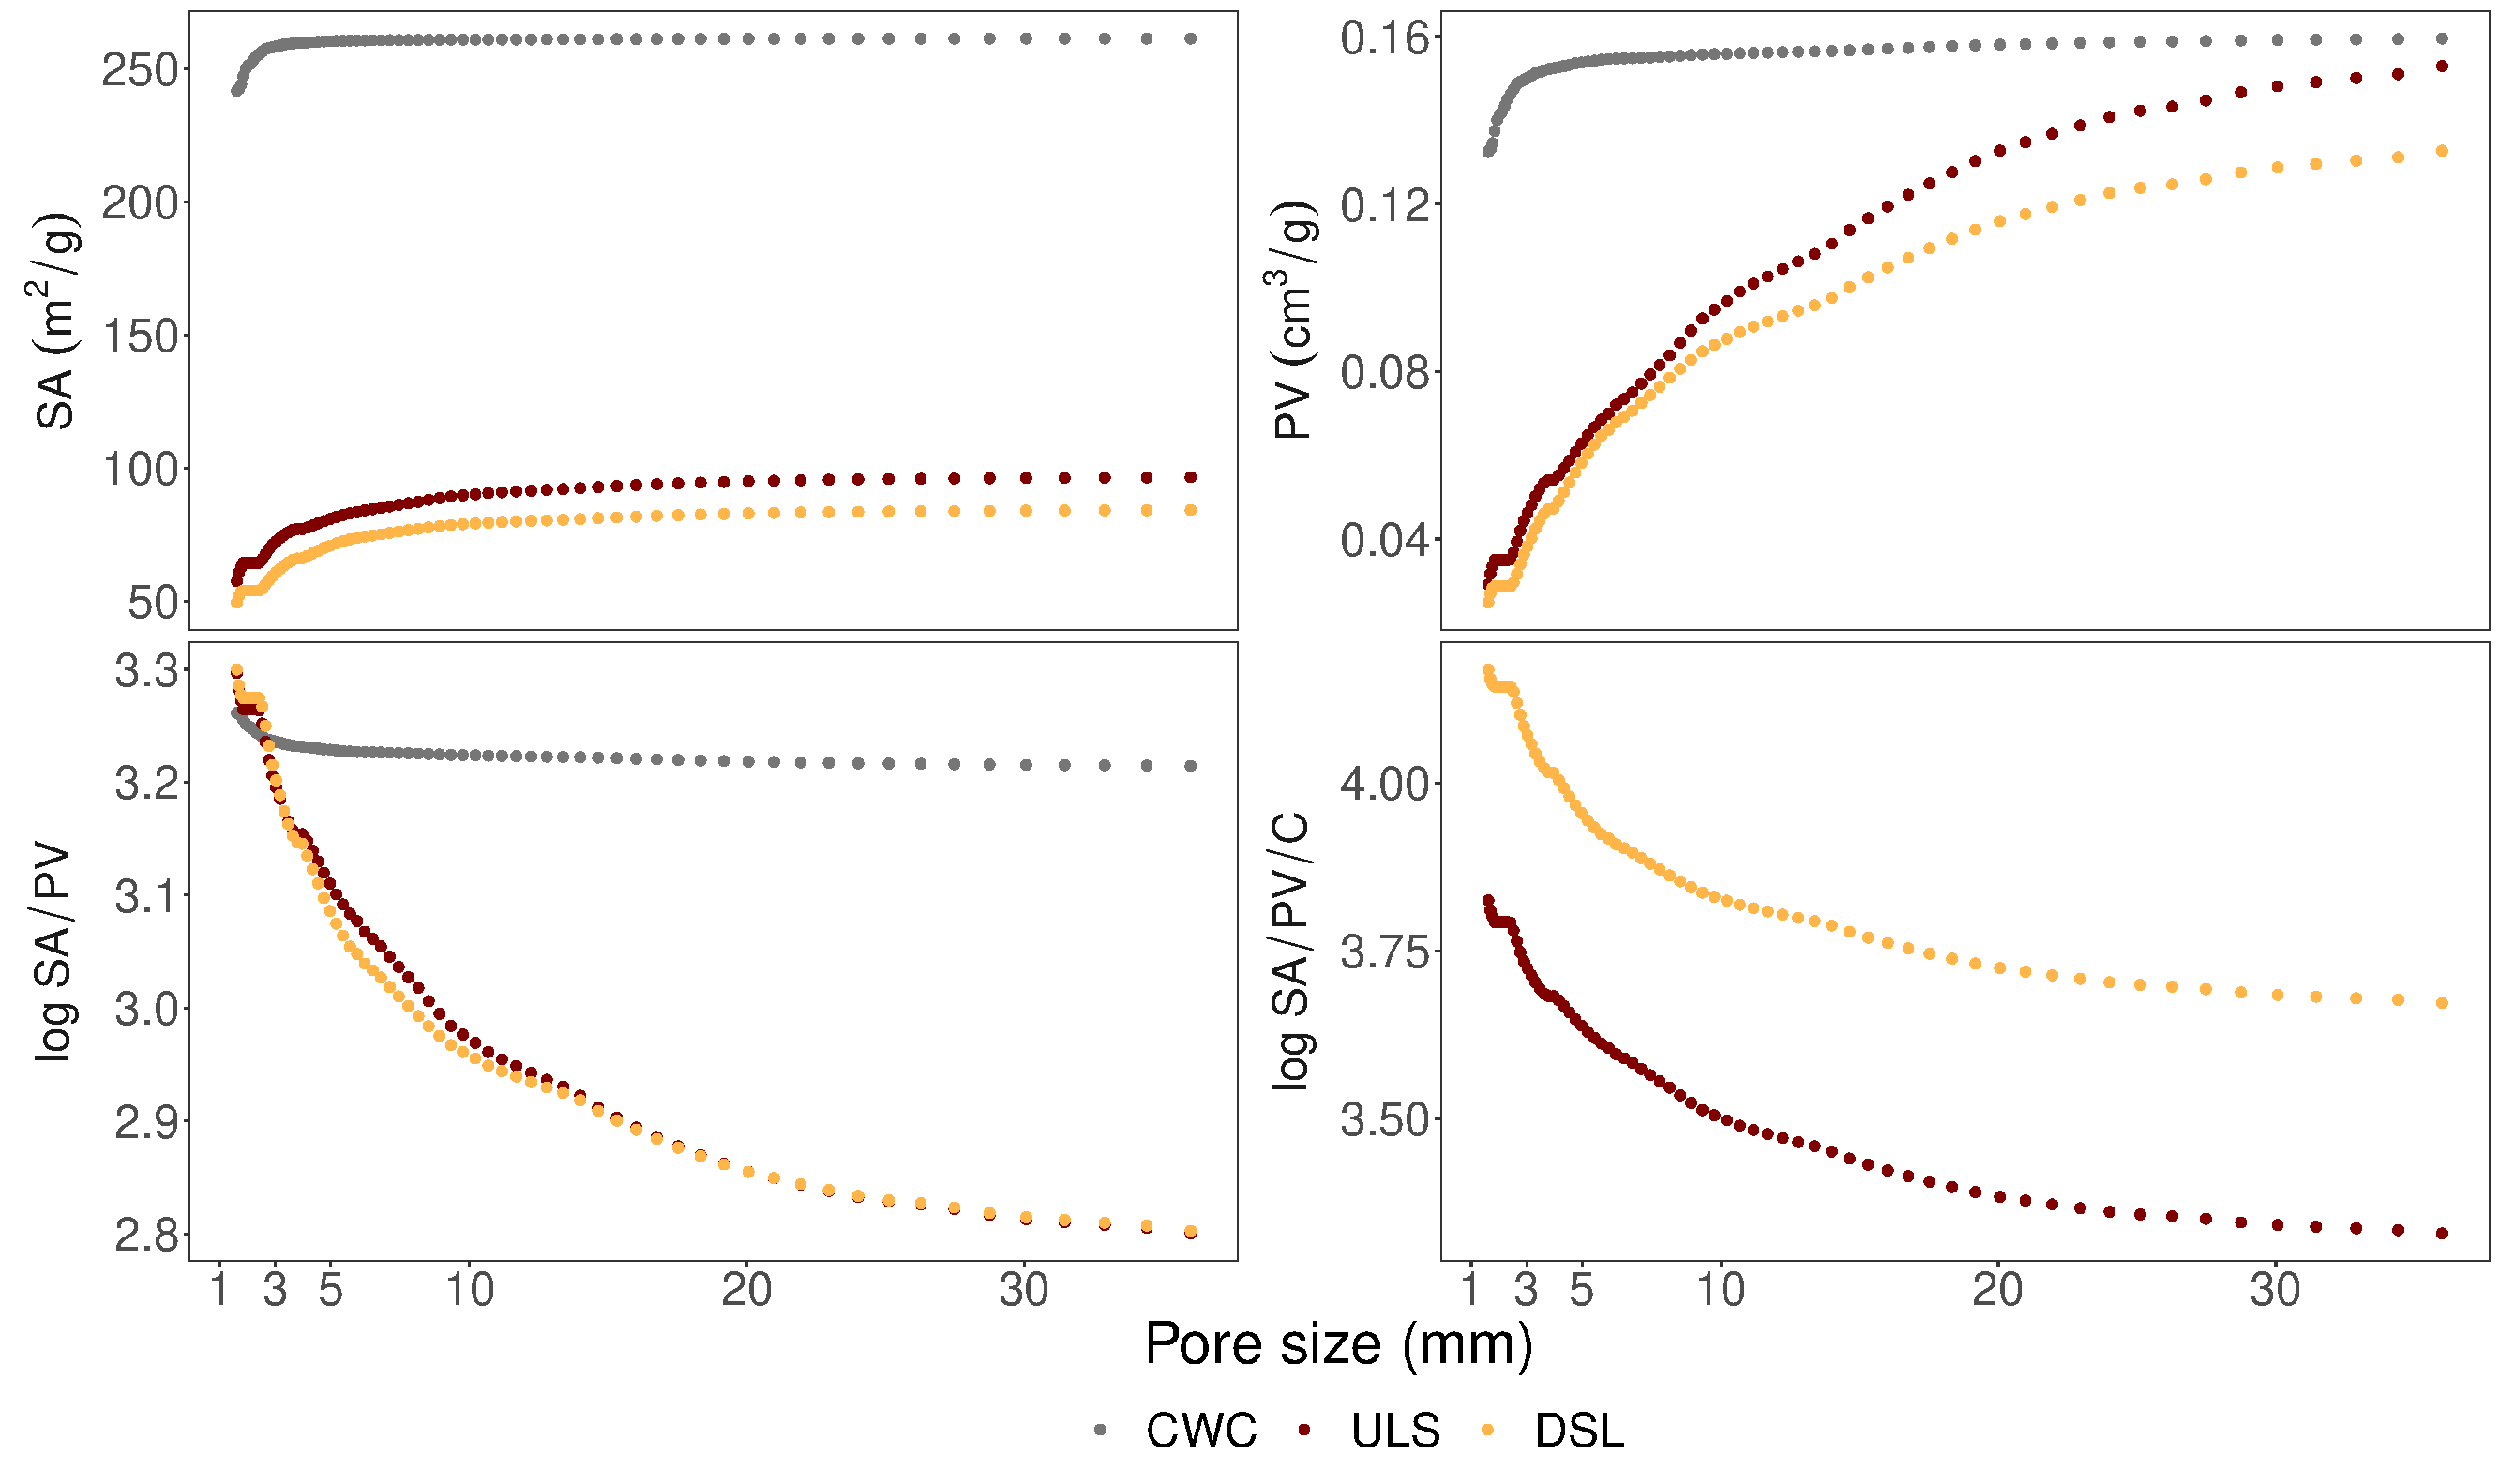
\includegraphics[width=\textwidth]{R/figs/PZD_SAPV_C_large.pdf}
    \caption{Cumulative pore size distribution for pores $>$ 1.5 nm using DFT theory. (a) Surface area, (b) pore volume, (c) SA/PV ratio for pores $>$1.5 nm normalized to carbon content (g C/g BC). (d) A lower SA/PV/C ratio indicates a higher degree of C in the pore wall matrix.}
    \label{fig:PZD_large}
\end{figure}


\subsection{Surface chemistry}
Based on feedstock type for the three biochars studied in this thesis, carbon content of the biochars follows the expected trend, CWC \textless ULS \textless DSL with 91.4\%, 29.6\% and 13.5\%, respectively (\cref{tab:SAPV}). Oxygen content was highest for DSL and ULS (61.4 and 57.1 \% respectively) compared to 5.5 \% for CWC. CWC has a low O/C and H/C ratio (\textless 1) whereas ULS and DSL have ratios \textgreater 1. A low H/C and O/C ratio is associated with high degree of aromaticity and few functional groups. This shows that the CWC matrix is dominated by aromatic carbon whereas ULS and DSL are dominated by oxidized carbon resulting in a more hydrophobic surface of the high-C biochar. The proportion of elements other than C, O, H and N contained in the biochar matrices is significantly lower for the clean wood biochar (1.4 \%) compared to the sludge biochars (10.9 and 23.2 \%), containing a greater mixture of other elements. Total elemental composition of the biochars is given in \cref{appSec:elements}. The results from this study is in contrast to literature \citep{Hale2016,Sormo2021,zhang2021sorption} that report that the sorption strength of organic compounds to biochar increases with decreasing biochar O/C and biochar H/C ratios. Thus, the higher sorption onto ULS and DSL cannot be explained by the sorbent composition of main elements alone.

\begin{figure}[htb]
    \centering
    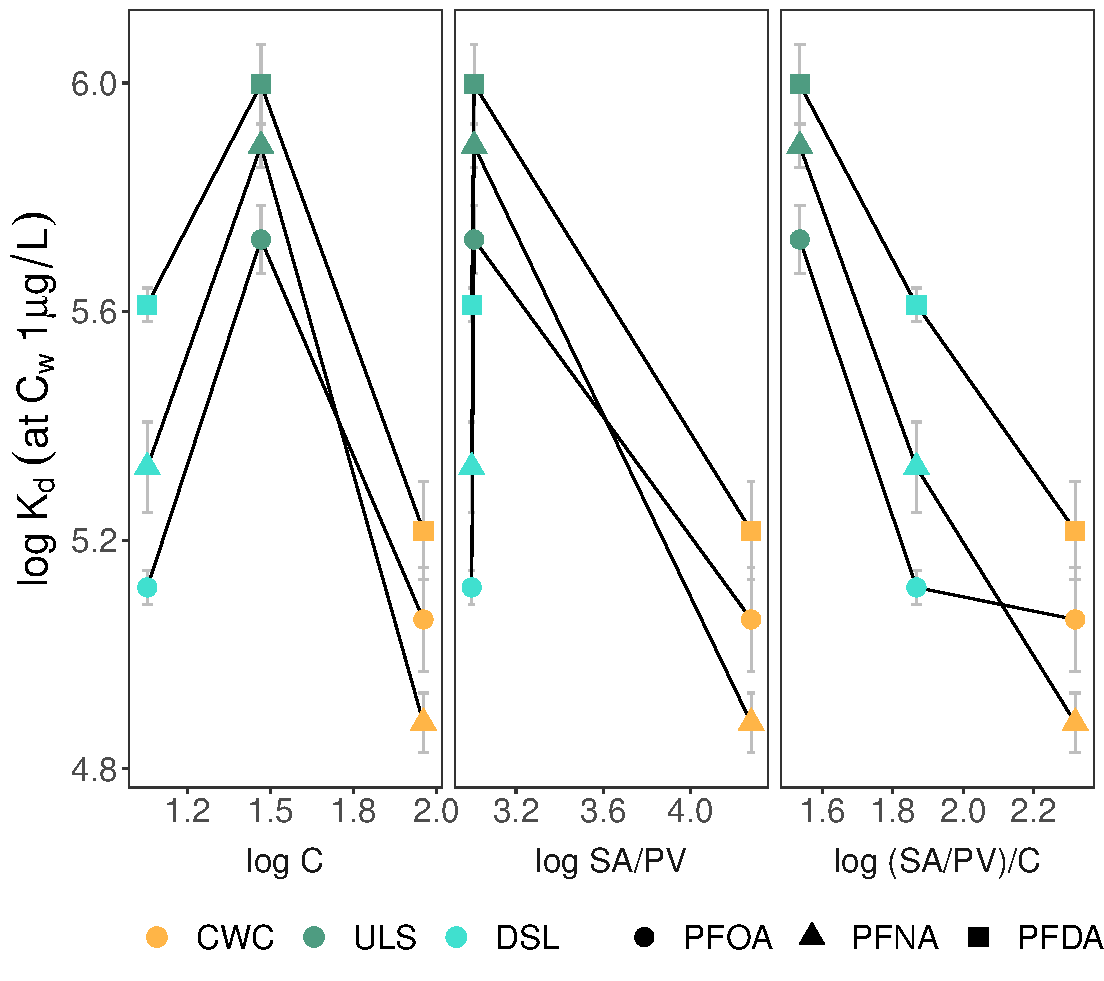
\includegraphics[width=\textwidth]{R/figs/SAPV_C_Kd1ugL_plot.pdf}
    \caption{The correlation of $log~K_d$ vs. (a) log C (b) log SA/PV (c) log (SA/PV)/C using BET for SA and BJH for PV by biomass feedstock. Error bars are the propagated standard error of $log~K_F$ and $n$.}
    \label{fig:Kd_SAPV_C}
\end{figure}


\subsection{Effect of solution chemistry}

\begin{table}
\centering
\caption{Composition of a selection of elements in the biochar samples in mg/kg.}
\label{tab:BC_mainElements}
\begin{tabular}{lllllllll} \toprule
 & Ca & Fe & K & Mg & Na & P & S & Si \\ \midrule
CWC & 8.03 & 0.13 & 4.0 & 0.91 & 0.052 & 0.41 & 0.089 & 0.17 \\
DSL & 26 & 180 & 3.7 & 4.7 & 1.8 & 8.0 & 7.2 & 0.62 \\
ULS & 21 & 23 & 6.8 & 5.3 & 2.4 & 45 & 2.9 & 1.7 \\ \bottomrule
\end{tabular}
\end{table}

\subsection{Effect of inorganic ions}
Elements that may affect sorption properties of the biochars are provided in \cref{tab:BC_mainElements}. Since ionic forms have not been analyzed, an assumption based on the total element composition must be made during the discussion of potential roles of inorganic ions for PFAS sorption. The sludge chars have expectantly the highest mineral content overall due to the heterogeneous composition of sewage sludge. 

Coexisting inorganic cations and anions complicates sorption behavior of PFCAs, where several mechanisms are involved in changing both solution and biochar surface chemistry \citep{du2014adsorption}. The presence of ions can both enhance or suppress sorption through mechanisms such as electrical double-layer compression, surface-charge neutralization, divalent cation bridging, competitive adsorption, and salting-out. The latter mechanism occurs only at high enough salt concentration and is not applicable for the present study. 

ULS and DSL are similar in earth alkali composition that gives rise to divalent ions  and CWC is one and two orders of magnitude lower in Ca and Mg, respectively. The presence of electrolytes creates an electrical double layer (EDL) that changes the adsorption surface. Divalent ions such as Ca\textsuperscript{2+} and Mg\textsuperscript{2+} in the EDL can function as bridges between the negatively charged functional groups of PFAS and surface negative charges. This divalent cation bridging effect has shown to be an important sorption mechanism in sediments, mineral materials, and black carbon, among others \citep{higgins2006sorption}. Apart from playing a bridging role between the BC surface and PFAS functional groups, divalent ions can function as intermolecular PFAS bridges which further enhances PFAS hydrophobicity by this complexation into larger molecules. Both Ca\textsuperscript{2+} and Mg\textsuperscript{2+} have been reported to play a role for chaining of perfluorinated carboxylic acids \citep{wang2011}. The role of divalent cations  

Increase in zeta potential 

Previous research suggests that calcium content is an important parameter contributing to stronger sorption of anionic organic molecules \citep{higgins2006sorption,sigmund2022sorption}. In this study, PFAS sorption to sludge enhanced with increasing calcium concentration in solution, divalent ions contribute to stronger sorption compared to monovalent ions due to ion bridging between negatively charged PFAS and biochar at low pH \citep{zhang2013sorption,arvaniti2014sorption,arvaniti2015review}. 

Do I have data on \% ash for each sorbent?
\begin{figure}[htb]
    \centering
    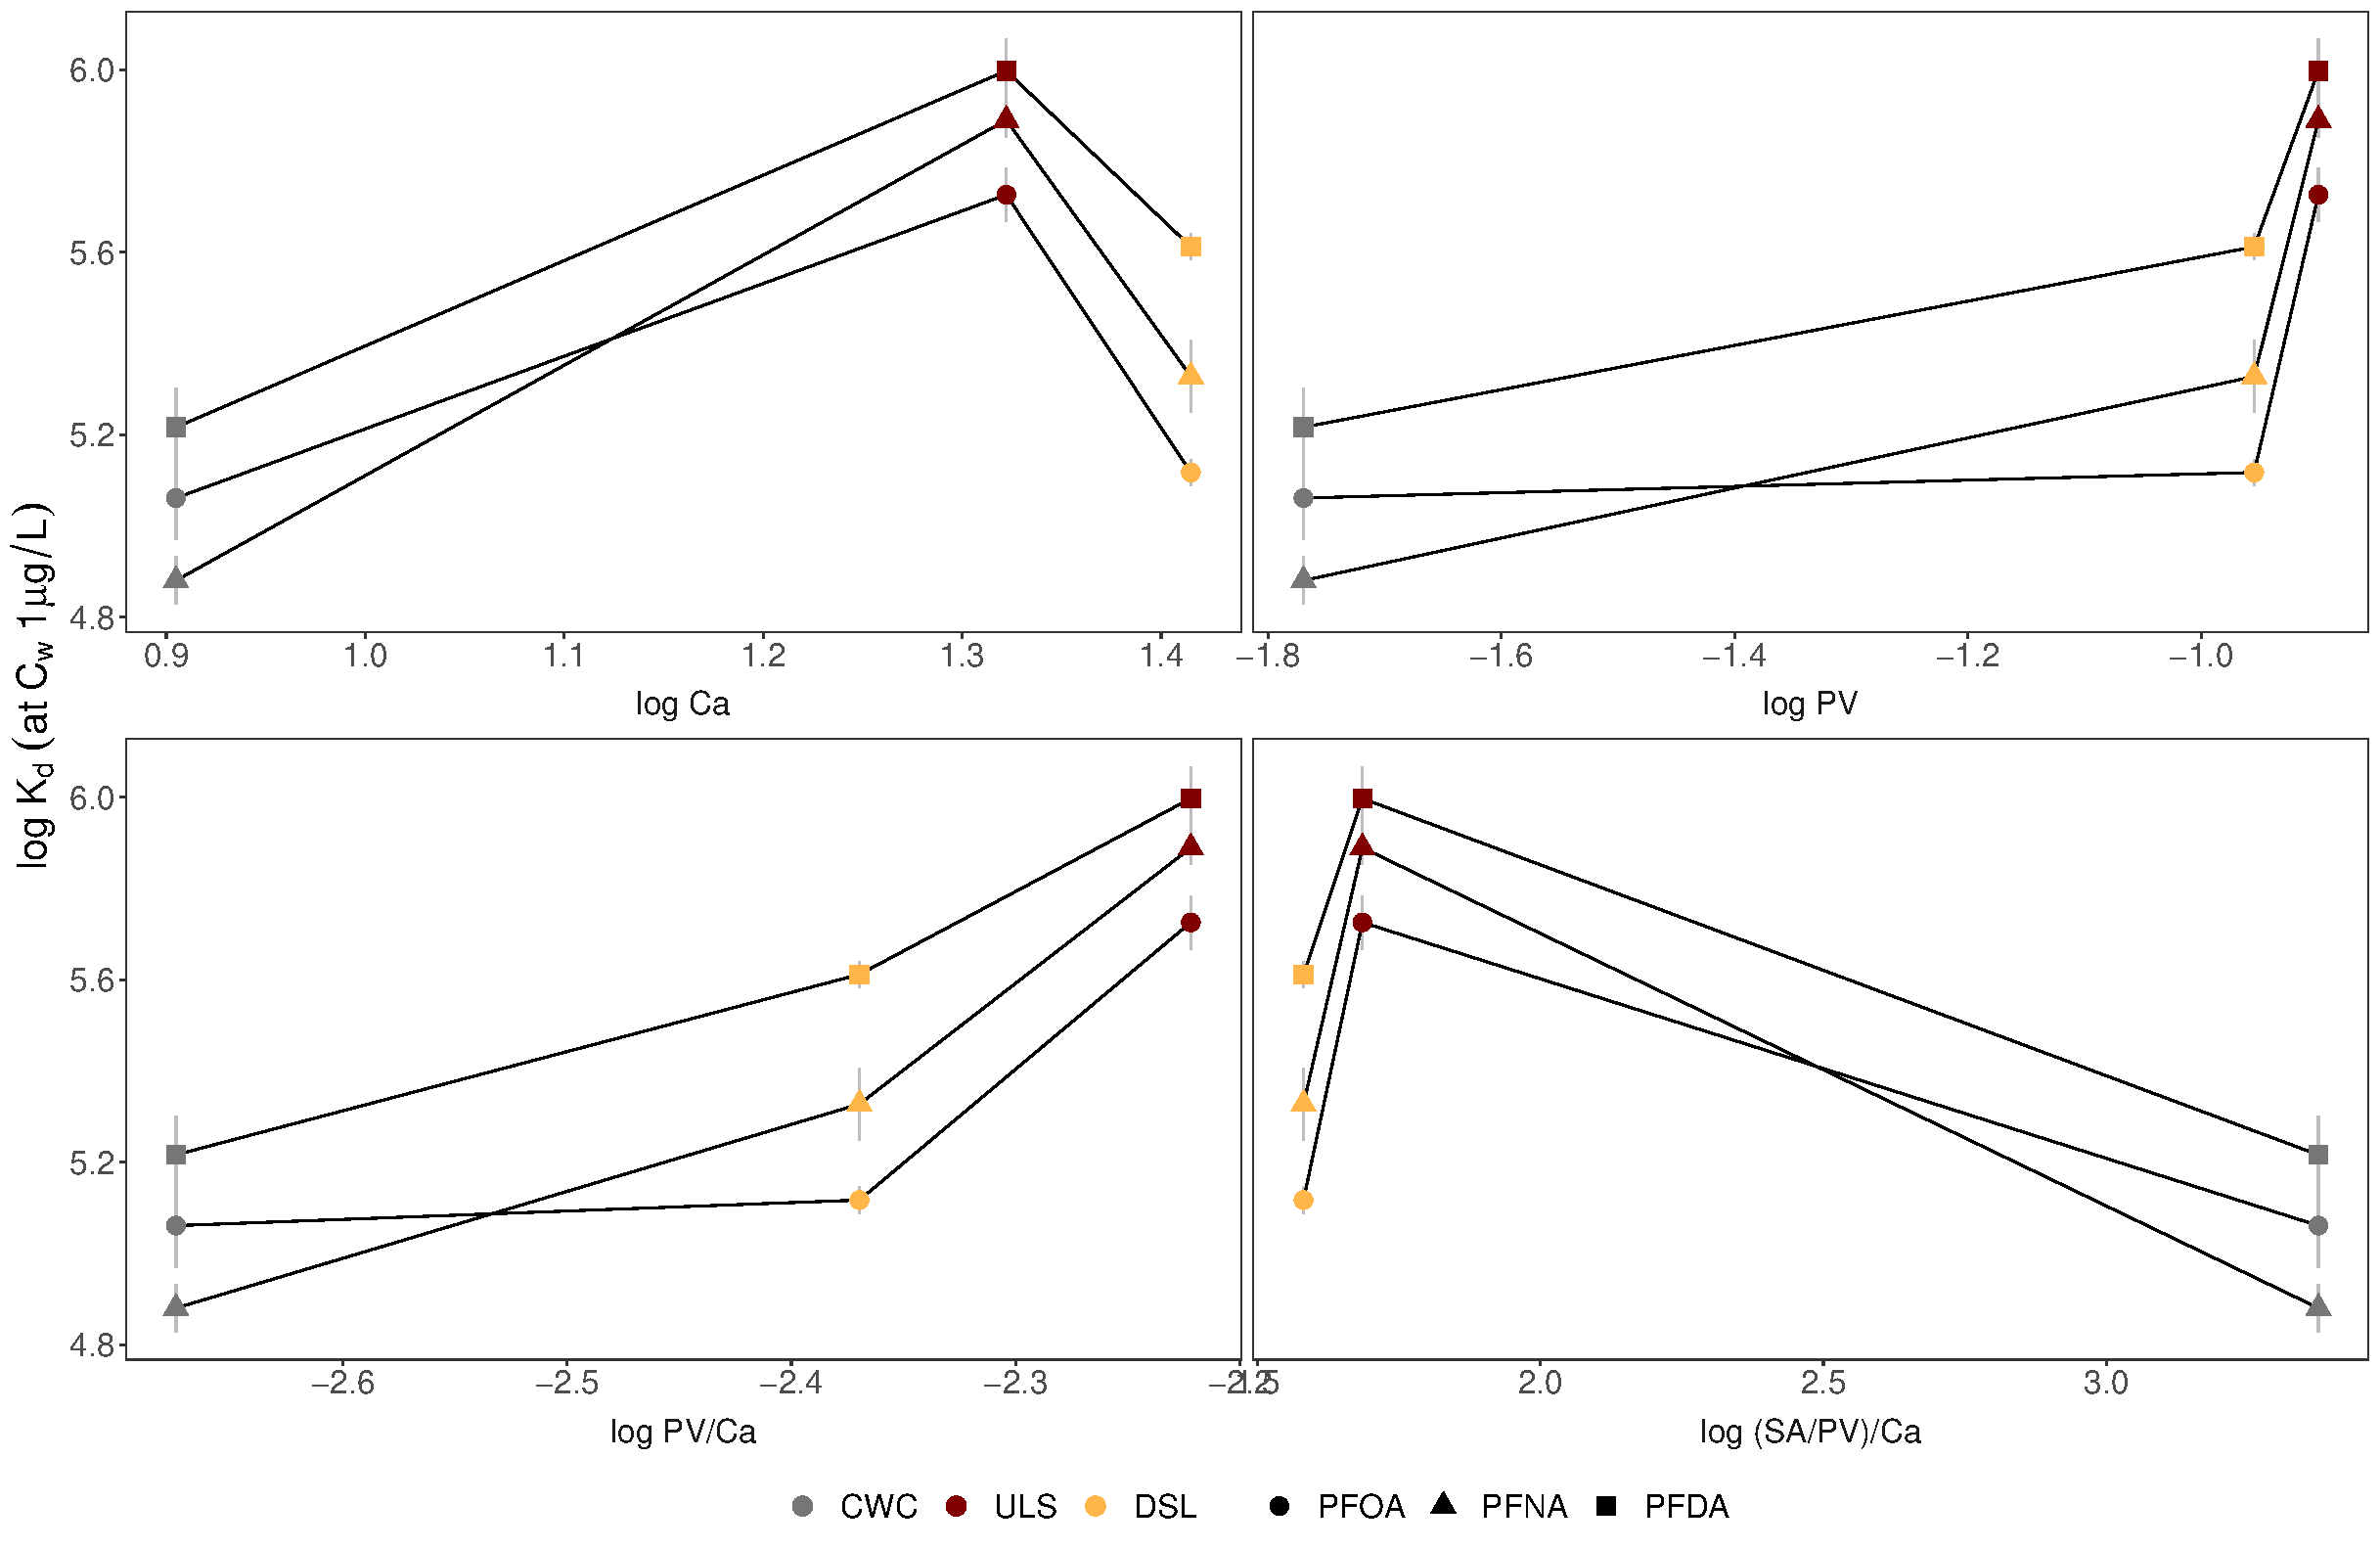
\includegraphics[width=\textwidth]{R/figs/Correlation_SAPV_Ca_plot.pdf}
    \caption{The correlation of $log~K_d$ vs. (a) log Ca (b) log PV (c) log PV/Ca (d) log (SA/PV)/Ca using BET for SA and BJH for PV by biomass feedstock. Error bars are the propagated standard error.}
    \label{fig:Kd_SAPV_Ca}
\end{figure}


Iron speciation, Synchrotron results, Inner-sphere complexes (covalent metal-ligand bonds) with Fe-carboxylate by ligand exchange \citep{gao2012adsorption}(NEED TO GET ACCESS TO ARTICLE, BUT CITED IN \citep{du2014adsorption}):

\begin{equation}
    \mathrm{\equiv Fe-OH_2^+~ + ~ CF_3(CF_2)_nCOO^- \rightarrow   ~ \equiv Fe-OOC(CF_2)_nCF_3 ~+~ H_2O}
\end{equation}

\subsection{Effect of solution pH and conductivity}
Adsorption capacity has shown to also be related to solution pH, which is expected to increase with decreasing pH \citep{du2014adsorption}. However, in Ca and Mg-rich basic solutions, sorption can be enhanced through divalent cation bridging effect. pH varied little between all biochar-soil-water systems with an average pH of 7.18 \textpm 0.02. Conductivity was 39 \textpm 0.9 \textmu S cm\textsuperscript{-1}. Since the variance is low, pH and conductivity was not considered as factors that influence sorption of PFCAs. The conductivity of soil-water samples differed the most from the rest of the samples with a mean conductivity of 23 \textpm 0.05 \textmu S cm\textsuperscript{-1} versus a mean of 41 \textpm 0.9 \textmu S cm\textsuperscript{-1} for the biochar-water and biochar-soil-water samples. Complete pH and conductivity data is in \cref{appSec:misclab}.

\citep{zhang2013sorption}: sorption of PFAS increases with decreasing pH

\begin{table}
\centering
\caption{Mean pH and conductivity (\textmu S cm\textsuperscript{-1}) measurements for the different batch test systems (n=3). The error bars represent the standard error. BC/S/L is the biochar:soil:liquid ratio.}
\label{tab:pHcond}
\begin{tabular}{lccccc}
\toprule
 & \multicolumn{2}{c}{pH} & \multicolumn{2}{c}{Conductivity} & \\ \cline{2-5}
 & mean & std. dev & mean & std. dev & BC/S/L\\ 
\midrule
ULS & 7.10 & 0.04 & 45.70 & 3.03 & 1/0/500\\
DSL & 7.31 & 0.02 & 40.93 & 1.07 & 1/0/500\\
CWC & 7.36 & 0.07 & 46.47 & 0.70 & 1/0/500\\
ULS+S & 7.18 & 0.02 & 34.93 & 0.40 & 1/50/500\\
DSL+S & 7.14 & 0.00 & 35.73 & 1.50 & 1/50/500\\
CWC+S & 7.09 & 0.05 & 44.90 & 1.54 & 1/50/500\\
S & 7.08 & 0.05 & 23.33 & 0.87 & 0/1/10\\
\bottomrule
\end{tabular}
\end{table}


%%%%%%%%%%%%%%%%%%%%%%%%%%%%%%%%%%%%%%%%%%%%%%%%%%%%%%%%%%%%%%%%%%%%%%%%%%%%%%%%%%%%%%%%%%%%%%%%%%%%%%%%%%%%%%%%%%%%%
%%%%%%%%%%%%%%%%%%%%%%%%%%%%%%%%%%%%%%%%%%%%%%%%%%%%%%%%%%%%%%%%%%%%%%%%%%%%%%%%%%%%%%%%%%%%%%%%%%%%%%%%%%%%%%%%%%%%%
%%%%%%%%%%%%%%%%%%%%%%%%%%%%%%%%%%%%%%%%%%%%%%%%%%%%%%%%%%%%%%%%%%%%%%%%%%%%%%%%%%%%%%%%%%%%%%%%%%%%%%%%%%%%%%%%%%%%%

\section{Potential for commercializing sludge chars as sorbents}
Potential challenges with application of sewage sludge-based sorbents: leaching of heavy metals, sorption capacity, pH (although liming raises pH which is not good for sorption, addition of Ca\textsuperscript{2+} creates divalent bridging effect and complexation of PFAS molecules that enhance sorption. 

Removal efficiency, good enough for application?

Leaching of heavy metals results at PT 700 C
    As, Cd, Co, Zn, Pb for all chars Below EBC limits, Cr and Ni between lower and upper limit
    EBC = European Biochar Certificate
    Cu above EBC limits for ULS and DSL
    Enrichment factors heavy metals (?)

\subsubsection{Field conditions representativeness}

Equilibrium conditions vs laboratory batch tests
BC dose

Are the results representative of what goes on in real life? Sorption by shaking for 14 days represent an assumed equilibrium between PFCAs in the water and soil phase. A comparable situation in the field would be washing of the soil with large amounts of water such as during heavy rainfall. This will only be the case during occasional stormwater events and thus the results from this research could benefit from being supplemented with results from leaching tests using biochar mixed with soil. However, the relationship:

\begin{align}
    \frac{k_1}{k_2}
\end{align}

where \(k_1\) is the PFCA sorption (adsorption and absorption) rate and \(k_2\) is the PFCA desorption rate, where \(k_1>>k_2\), which indicates that sorption is many times higher, and in an equilibrium situation, sorption and desorption will be at steady state \citep{Cornelissen2005}. 

\section{Sustainability}
\subsection{Life cycle impact assessment (LCIA)}
LCA (life cycle assessment), sustainability aspects of production of biochar
High operating energy and cost different technologies \citep{Alhashimi2017}
Energy demand pyrolysis 

\section{Quality control of laboratory analysis and uncertainty}
Standard concentration (but at least leads to underestimation of results)
\subsection{Spiking standard concentrations}
SPE and directly, why?

The pipettes used for making the PFCA dilutions were calibrated. The three pipettes were: 1) 2-10 mL, 2) 200-1000 \textmu L, and 3) 5-50 \textmu L. All pipettes were below the permitted coefficient of variation (CV = 0.3, 0.5, and 2 $\%$ respectively (\cref{appSec:misclab}, \crefrange{appTab:pip2-10}{appTab:pip5-50}).

Since the diameter of the centrifuge tube (30 mm) was larger than that of a volumetric flask and biochar was added prior to the dilution process, the final concentration of the sorbent-sorbate mixture may have a heightened inaccuracy. However, the volume of which 0.1 g biochar occupies can be considered insignificant due to the high absorptive capacity of biochar and small mass used. Therefore a set of 10 centrifuge tubes filled to 50 mL containing 0.1 g CWC were weighed to control the uncertainty of the final dilutions. The results from weighing show that the weight of 10 trials were not accurate but precise, which means that all samples were prepared with the same final volume even though this volume deviates from 50 mL (\cref{appTab:PPcentrifuge}). 

Volume 50 mL weighed vs by eye measurement, diameter of test tube and error
preparation of cocktail standard, not consistent, some individual pipetting. 

\subsubsection{Filter blanks no significant difference}

\subsection{PFAS losses during laboratory analysis}
SPE protocol, many steps, many PP test tubes transfers, saturated PFAS-solutions, internal standard (dilutions had to disregard IS because too low concentration)

\citep{Lath2019labsorb}: 
Syringe filters: sorption of PFOA to centrifuge tubes and filter membranes. Sorption onto syringe surface: negligible due to short residence time (\textless 10 s). 74\% recovery from regenerated cellulose syringe filter. No improvement in recovery was seen when conditioning the syringe filters with phosphate solution or methanol. No trend between losses of PFOA on syringe filter and increasing spike concentrations. Centrifugation only is therefore advised if possible to avoid filtration losses. 

Test tubes: Greater recoveries from glass tubes than plastic, PP poorest recovery (55-68 \% recovery)... Contact time of PFAS residing in tubes for longer than 7 days should not be of significance, as \citep{Lath2019labsorb} propose that sorption and saturation of tube walls occur within hours. 74-81 \% recovery for PP when testing dependence on pH and ionic strength. Slight pH dependence, higher recovery at higher pH due to repulsion of negatively charged functional groups (PP has negative surface charge above pH 3.5-4. Bridging effect will be observed at higher pH's between cations like Ca2+, but is still considered negligible compared to the losses due to the physicochemical properties of the materials themselves. In general PP and plastics consists of mainly carbon hydrogen chains and are more hydrophobic than glassware. Sorption to tube walls saturate, so recoveries increase significantly with higher spike concentrations (e.g. for PP, 12-415 ug/L spiked PFOA increased recovery from 53.7-85.5 \%). Therefore, quantification of low concentrations may be subject to highest error, and in most cases will be an underestimation of dissolved concentrations. 

Use of PP test tubes, study
Higher probability of underestimating Cw for low-concentration samples because tube walls saturate – maximum number of sorption sites, there is a sorption maximum (Langmuir)

\subsection{Uncertainty}
\subsubsection{Batch tests}
Vel, du kan jo prøve å legge sammen alle de feilene. Det finnes jo forskjellige typer feilkilder i et stort forsøksoppsett. Det man ofte ser er at det er en eller to feil som er så store at de overskygger de andre. Da er det ikke noen vits å ta med alle de små. Feilen som ofte er størst er reproduserbarhet av metoden. Altså forskjellen mellom for eksempel prøver laget i triplikater. Det du kan gjøre i oppgaven din er jo å kort diskutere feilkildene du har og identifisere de største og viktigste.

\subsubsection{Analytical}
Calibration curves and matrix effect, 3-point curve
LC-MS/MS

\subsubsection{Peak integrations}
Manual review of peak integrations
decisions to remove C1 at low signal
where observed similar peak integrations across concentrations, suspected saturation of detector, dilution of these samples